\documentclass[11pt]{report}

\usepackage{geometry}
 \geometry{
 a4paper,
 total={210mm,297mm},
 left=25mm,
 right=25mm,
 top=30mm,
 bottom=25mm,
 headsep=7mm}

\interfootnotelinepenalty=10000

\usepackage[dvipsnames]{xcolor}
\usepackage{graphicx}
\usepackage{titlesec}
\usepackage{todonotes}
\usepackage{float}
\usepackage[hidelinks]{hyperref}
\usepackage{listings}
\usepackage{enumerate}
\usepackage{fancyhdr}
\usepackage{longtable}

\graphicspath{ {images/} }

\pagestyle{fancy}
\fancyhf{}
\fancyhead[L]{\leftmark}
\fancyfoot[C]{\thepage}
\renewcommand{\headrulewidth}{0.4pt}

\begin{document}

	\begin{titlepage}
		\centering
		
\includegraphics{logo.png}\par\vspace{1cm}
		{\scshape\LARGE\bfseries Politecnico di Milano \par}
		\vspace{1cm}
		{\scshape\Large Software Engineering 2\par}
		\vspace{1.5cm}
		{\Huge\bfseries Design document\par}
		\vspace{1cm}
		{\small Version 1.0 - 26/11/2017\par}
		\vspace{4cm}
		{\Large\itshape Pietro Melzi, Alessandro Pina, Matteo Salvadore\par}

		\vfill

		% Bottom of the page
		{\large AA 2017-2018\par}
	\end{titlepage}

	\tableofcontents{}

	\chapter{INTRODUCTION}
	\label{ch:INTRODUCTION}
	
		\section{Purpose}
		\label{sect:Purpose}
			\todo{TODO}
			
		\section{Scope}
		\label{sect:Scope}
			\todo{TODO}
			
		\section{Definitions, Acronyms, Abbreviations}
		\label{sect:Definitions, Acronyms, Abbreviations}
			\subsection{Definitions}
	\begin{itemize}
	\item \textit{Arrange trip}: the system provides all the information available about a travel to the user. If the travel is related to one or more public travel means, the system helps the user to organize it. It is indicated if the user already holds a valid ticket for a certain travel or if he has to buy a required one. Purchase of a ticket is handled on the websites of the transport service providers. Trip and travel are synonymous.
	\item \textit{Best path}: it is the preferred travel option proposed to reach the event location among all the feasible paths, according to parameters specified by the user. The best path can be chosen according to one of these features: length, cost or environmental sustainability. Best path is the path taken into account and showed in the daily schedule; the user can substitute it at any moment with an alternative feasible path. 
	\item \textit{Break event}: it is an optional event whose starting and ending time are flexible. The user can define this kind of event when he wants to reserve a certain amount of time in the schedule and he doesn't need to specify a starting time. For instance, a user could be able to specify that lunch must be possible every day between 11:30-
2:30, and it must be at least half an hour long, but the specific timing is flexible. The app would then be sure to reserve, if possible, at least 30 minutes for lunch each day.
	\item \textit{Constraint}: it is a rule defined on travel means by the user. When the system calculates feasible paths, each constraint must be taken into account: travel options not respectful of existing constraints are ignored. A constraint can be associated to a type of event. 
	\newline
	There are different types of constraints: min/max distance allowed for a travel mean, interval of hours in which it is possible to take a travel mean and possibility to deactivate a travel mean. 
	\item \textit{Customized type of event}: it is a set of rules related to a particular type of event that can be used several time by the user. The user can define a customized type of event in hs preferences, starting from the default type of event.	
	\item \textit{Default type of event}: it is a general set of rules defined usually the first time that the user exploits the system, it can be modified. Default type of event is related to each event that doesn't need a particular type of event. New types of event are defined starting from the constraints enclosed in the default one.	
	\item \textit{Feasible path}: a path that allows the user to reach a specified location before the starting time of the event to attend. It observes the constraints defined for that event.
	\item \textit{Google Maps API}: a set of functions offered by Google Maps to decide the travel path between two locations.
	\item \textit{Overlapping event}: an event (or a part of it) that happens in the same time slot of another event, added previously in the schedule. Because the schedule must be feasible, an event is considered as "overlapping" also if only its related travel overlaps an event present in the schedule.
	\item \textit{Periodicity}: it is related to events that occur more than one time. It can be defined as weekly, monthly or in which days of the week the event happen.
	\item \textit{Schedule}: a daily plan containing a set of events inserted by the user that allows him to travel and attend all the events. If an event overlaps other events, it cannot be inserted into the schedule. 
	\item \textit{Type of event}: a set of rules (constraints) that is defined by the user and can be associated to multiple events.
	\item \textit{Transport service provider}: a public or private company that controls and supplies the transport with a travel mean. 
	\item \textit{Travel}: it is used to indicate the path that the user has to follows in order to reach a location. It can be composed by different travel components.
	\item \textit{Travel component}: each single path that can be traveled with a travel mean. It has a starting time, a ending time, a departure location, an arrival location and a length. The union of one or more travel components creates a travel.
	\end{itemize}
			\subsection{Acronyms}
	\begin{itemize}
	\item \textit{API}: Application Programming Interface;
	\item \textit{ACID}: Atomicity, Consistency, Isolation and Durability;
	\item \textit{DB}: Data Base;
	\item \textit{DBMS}: Data Base Management System;
	\item \textit{DD}: Design Document;
	\item \textit{GCM}: Google Cloud Messaging;
	\item \textit{GTFS}: General Transit Feed Specification;
	\item \textit{HTTP}: HyperText Transfer Protocol;
	\item \textit{ICSEA}: Tenth International Conference on Software Engineering Advances;
	\item \textit{ITD}: Implementation and Test Document;
	\item \textit{Java EE}: Java Enterprise Edition;
	\item \textit{RASD}: Requirement Analysis and Specification Document;
	\item \textit{RESTful}: REpresentational State Transfer;
	\item \textit{RSA}: Rivest-Shamir-Adleman algorithm;
	\item \textit{UTC}: Coordinated Universal Time.
	\end{itemize}
			\subsection{Abbreviations}
	\begin{itemize}
   	\item \textit{TSP}: Transport Service Provider. 
	\end{itemize}
\todo{TODO}
			
		\section{Revision history}
		\label{sect:Revision history}
			2017/11/26 - \textit{Version 1.0} - First delivery of DD.
			
		\section{Reference Documents}
		\label{sect:Documents}
			\begin{itemize}
\item Specification Document: "Mandatory Project Assignments.pdf";
\item Specification Document: "Implementation and Testing Assignments.pdf";
\item Requirements Analysis and Specification Document, version 1.1;
\item Design Document, version 1.1.
\end{itemize}
			
		\section{Document Structure}
		\label{sect:Document Structure}
			\todo{TODO}
			
	\chapter{ARCHITECTURAL DESIGN}
	\label{ch:ARCHITECTURAL DESIGN}
	
		\section{Overview}
		\label{sect:Overview}
			In this section we'll present a general overview of the system-to-be, with specific focus on the main logical components and their interactions.
The main high-level components of the system are:
\subsubsection{Mobile App:}
\label{subsubsect:Mobile App}
The presentation layer that let the users access the functionalities offered by the Travlendar+ on their smartphones. The mobile app offers also an internal logic that handle:
\begin{itemize}
\item notifications reception, through Google Cloud Messaging APIs;
\item map displaying and path drawing through Google Maps mobile APIs.
\end{itemize}  

\subsubsection{Web Browser:}
\label{subsubsect:Web Browser}
The presentation layer that let the users access the functionalities offered by the Travlendar+ on their browsers.
It relies on the connection with the web server in order to obtain dynamic web pages.
\subsubsection{Web server:}
\label{subsubsect:Web server}
This layer provide web pages for the web-based application, it communicate directly with the application server interfaces to satisfy the client requests, using proper Interfaces. This layer interact also with an external system (Google Maps API) in order to display an embedded map containing the user travel's information.

\subsubsection{Application Server:}
\label{subsubsect:Application Server}
The logic layer that implements all core system's functionalities. It receive and reply to client's requests, if required it send notifications to the mobile applications, it interact with external systems in order to satisfy the user's requests and it interact with a DBMS in order to guarantee the information persistence.
In particular the application server will interact with:
\begin{itemize}
\item Google Maps APIs in order to provide feasible paths according to the user preferences;
\item Transport Service providers systems to provide trips arranging functionalities, such as ticket buying, location of sharing vehicles and strikes informations.
\item Weather APIs in order to provide weather informations and to apply possible travel constraints related to the weather.
\item Google Cloud Messaging APIs ino order to send notifications to the user's mobile Apps.
\end{itemize} 
\subsubsection{Database Server:}
\label{subsubsect:Database Server}
The data layer, that supports all data storage and management operations. This layer ensure that ACID properties are satisfied. The database server will interact only with the application server, the data will never be exposed directly to the client layers.
\subsubsection{External Systems:}
\label{subsubsect:External Systems}
This are not internal components of our application, but the system-to-be will have to interact with them in order to guarantee all the system functionalities.
Most of their interactions with the system are already been described in the previous paragraphs, but here we'll explain in detail the interaction with Transport Service providers: Travlendar+ will initially integrate some external transport service systems (public transport service providers and sharing vehicles provider) but will also offer proper API to allow others Transport Service providers to interact with Travlendar+ and so to be considered as suggested travel means to the users.


\begin{figure}[H]
\begin{center}
		\hspace*{-50pt}
		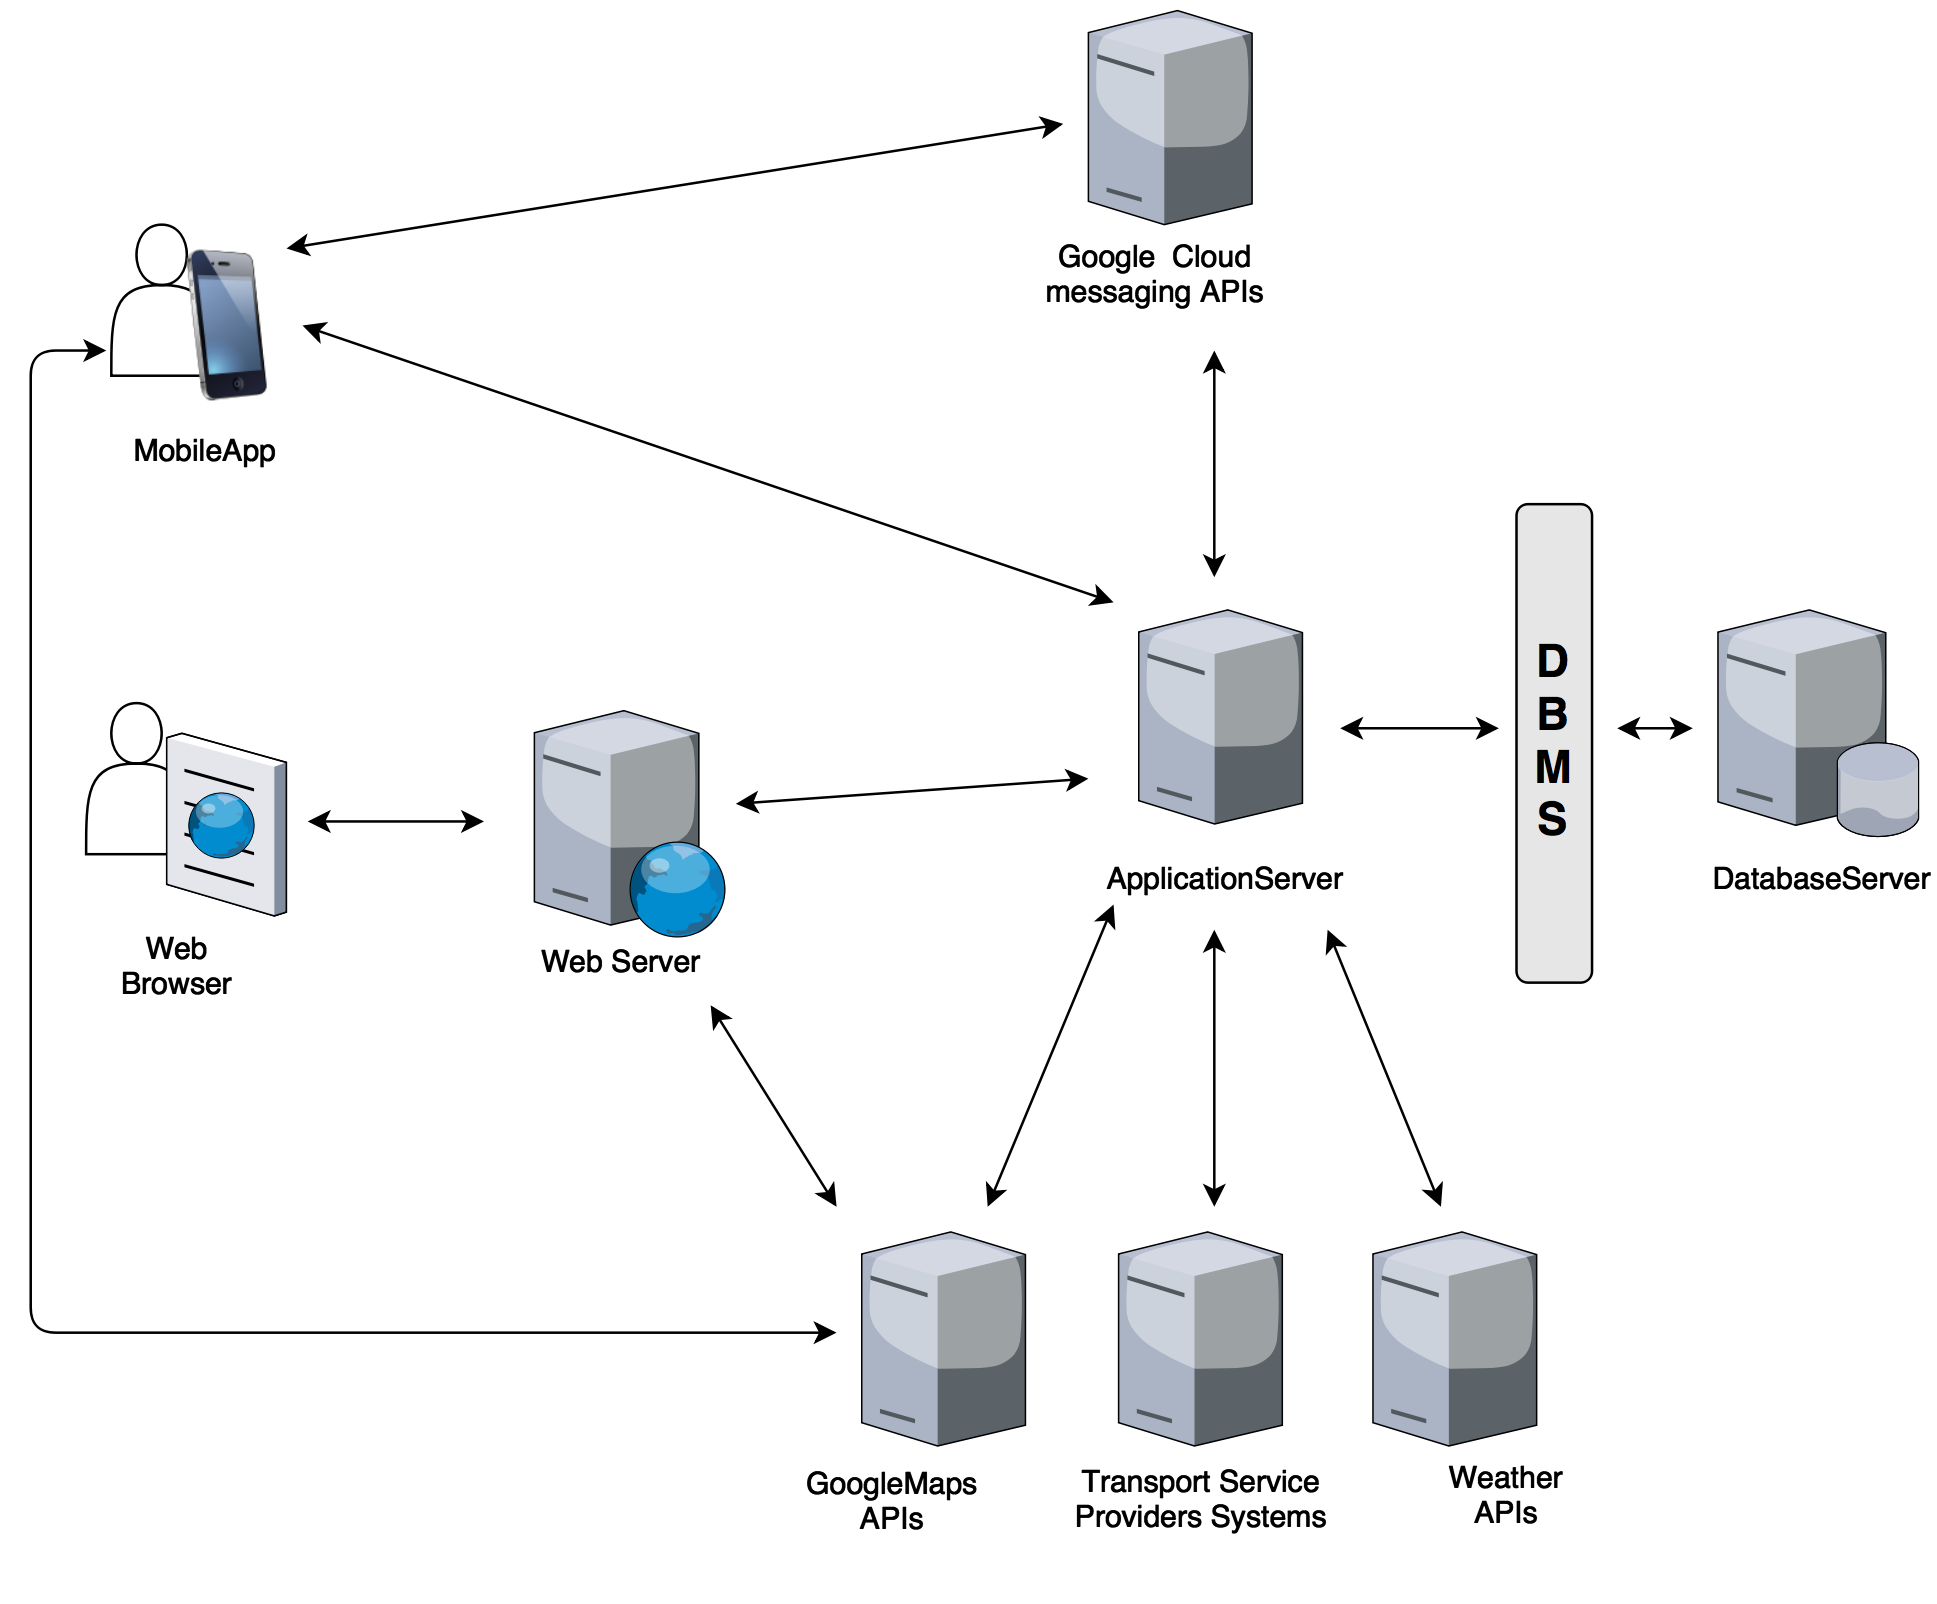
\includegraphics[scale=0.2]{GeneralArchitecture.png}
\end{center}
\caption{General Architecture}
\end{figure}

			
		\section{Component view}
		\label{sect:Component view}
			In this section we'll present and analyze the main components in which our system is divided and we'll explain the relations between them.
		
\subsection{Application Server}
\label{subsect:Application Server}
	\begin{figure}[H]
		\begin{center}
			\hspace*{-60pt}
			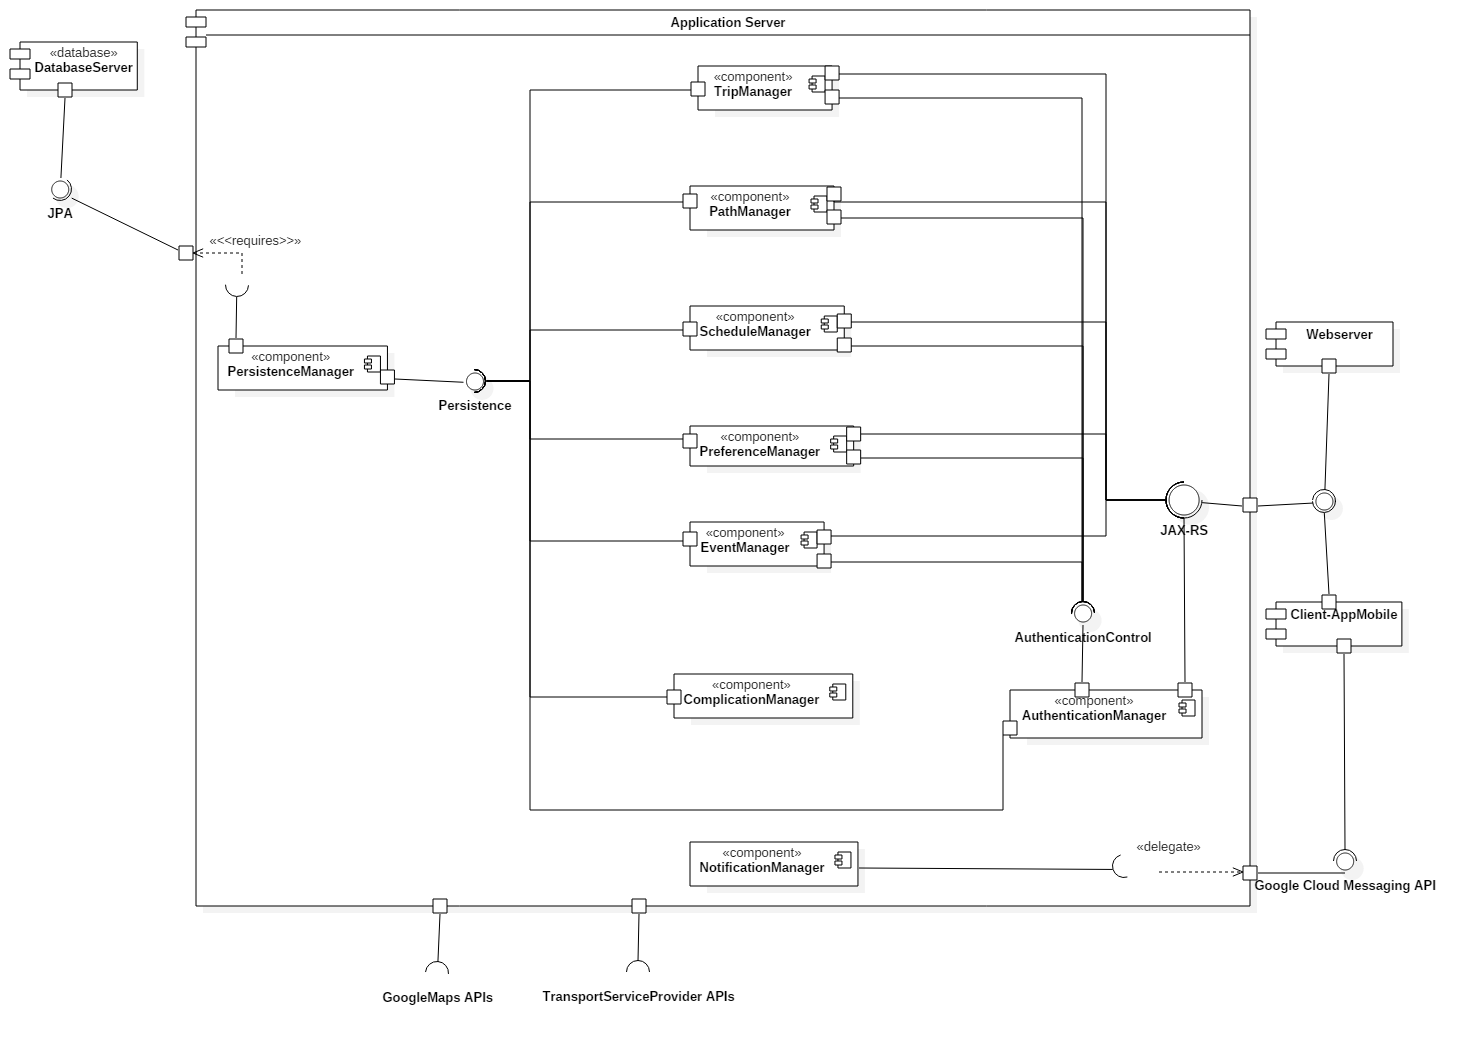
\includegraphics[scale=0.4]{ApplicationServer.png}
		\end{center}
		\caption{The components of the Application Server}
	\end{figure}
	The application server must handle the whole business logic of the application, the connection with the data layer and it must expose all the needed functionalities to the users. It also has to interact with external systems. \\ \\
The main application server components are:
\begin{itemize}
	\item \textbf{AuthenticationManager:} This module will manage the user registration, the user login and it will be involved in any user request to the application server in order to check if the request comes from an authorized device;
	\item \textbf{CalendarManager:} This subsystem will manage all calendar-related functionalities of Travlendar+'s system, its structure will be better explained in the dedicated section below, among with a schema of the internal components;
	\item \textbf{TripManager:} This module will provide the logic needed to arrange the users trips; to do so, this module will interact with external systems of Transport service providers in order to allow the user to buy public transportation tickets or to locate the nearest vehicle of a sharing system when those travel means are involved in the user's travel path;
	\item \textbf{ComplicationManager:} This module will periodically checks if the travels that are close in time are still feasible. To do so it will interact with external systems of Transport service providers to gain information about strikes, with open weather APIs to obtain information about the weather and with Google Maps APIs to obtain information about the traffic. If this module detects that a travel is no more a feasible one, it will charge the NotificationManager to warn the involved user;
	\item \textbf{NotificationManager:} This module will serve as a gateway to all the notifications to be sent, from others modules, to the user's mobile devices. To do so it will use the Google Cloud Messaging APIs in order to ensure a transparent interface with both IOS and android devices;
	\item \textbf{PersistenceManager:} This module will provide transparent access to the database functionalities from all the others modules. All system database functionalities must be developed inside this module;
\end{itemize}

\subsubsection{Calendar Manager}
\label{subsubsect:Calendar Manager}
\begin{figure}[H]
	\begin{center}
		\hspace*{-60pt}
		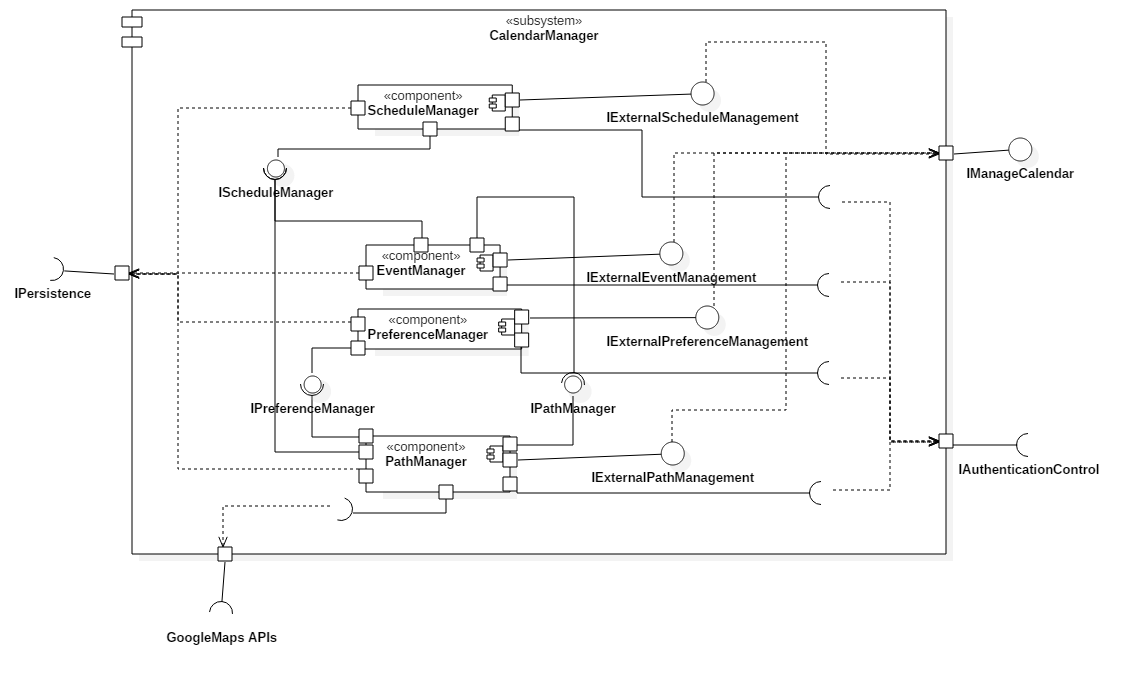
\includegraphics[scale=0.5]{CalendarSubsystem.png}
	\end{center}
	\caption{The components of the CalendarManager subsystem}
\end{figure}
	This subsystem will implement the core functionalities of our system, it is composed of four main components:
	\begin{itemize}
		\item \textbf{PathManager:} This module will manage the user travels computation, after the insertion or the modification of an event or also after a specific user requests to change a selected path. It will compute the feasible paths through the invocation of Google Maps API and it will also interact with the PreferenceManager in order to obtain the information needed to guarantee that the user preferences are respected in every proposed path. 
		\item \textbf{EventManager:} This module will manage the insertion, deletion and modification of the events into the user calendar. It will interact with the ScheduleManager in order to find out if an event does overlap with others events. When an event is created it will involve the PathManager in order to provide feasible paths to reach the inserted events. It will also handle insertion, deletion and modification of the flexible breaks. \\
	If the users has inserted one or more periodic events, this module will handle their propagation in the time. 
		\item \textbf{ScheduleManager:} This module will manage the event's scheduling functionalities: it is able to check if an event overlaps with others events and to guarantee that the flexible breaks are respected. It will also check that the user's travels does not overlap with other events. When an event overlaps with another one, it will put it in a separate list of non scheduled events and it will manage the user's requests of rescheduling these events.
		\item \textbf{PreferenceManager:} This module will offer all the functionalities needed to insert, modify and delete the user's event profiles. It will also interact with the module that has to apply the event profiles in order to compute the travel paths(PathManager).
	\end{itemize}
	
\subsection{Database}
\label{subsect:Database}
	\todo{TODO ER + description}

\subsection{Web Server}
\label{subsect:Web Server}
	The web server layer connects the users that wants to use Travlendar+ through a web browser with the Application Server. \newline
	The main functions to be implemented in this layer are basically interfaces.
	The only logic in this layer is used to embed a map into the relative web page and to draw the paths the user must travel to reach his events. To do so the web browser will interact with Google Polylines APIs.\newline
	The presentation will be handled by the JavaServerPages component that will be implemented using JSP pages. The interaction with the Application server and with the maps API will be handled by the WebController module.

\subsection{App Mobile}
\label{subsect:App Mobile}
	The web server layer connects the users that want to use Travlendar+ through their mobile devices with the Application Server.
	To do so it uses three main modules: the GUIManager will handle all the presentation functionalities of the app, the DBManager will handle all the users data, such as events and some information about travels duration, in order to enable the user to use some of the app functionalities even when he does not have access to an Internet connection, the ApplicationController will handle the interaction with the server, using the inputs provided by the users through the GUIManager and also requesting data manipulation operations in the local app database with the information received from the server. The application controller will also handle the notifications received and it will interact with Google Polylines APIs for mobile devices in order to to draw the paths the user must travel to reach his events and provide GPS path following functionalities.
	\todo{TODO E-R of the mobile database}
	
	
\begin{figure}[H]
\begin{center}
		\hspace*{-0pt}
		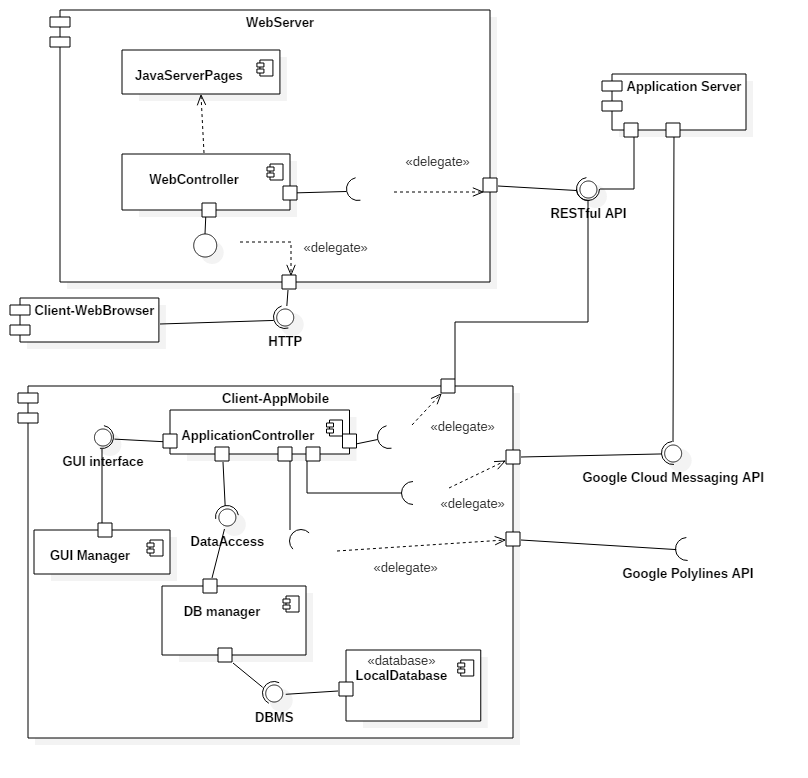
\includegraphics[scale=0.5]{Client_and_web_server.png}
\end{center}
\caption{The components of the web server, of the client app and of the client browser}
\end{figure}
\todo{TODO implementation choices in the Application server are still to be written}
Our implementation choice will be to use Java Enterprise Edition 7 (JEE)
In order to provide a mean to interface to the client and the web server the application server will use 
			
		\section{Deployment view}
		\label{sect:Deployment view}
			The main purpose of this section is to show how the various components of the system are actually deployed on the hardware infrastructure.\\
During the design process of the physical architecture are been taken into account both functional and non functional requirements. In particular we've focused on the following non functional requirements: reliability, availability and security. In order to satisfy those requirements we have identified the following 5-tiered architecture:
\begin{figure}[H]
\begin{center}
		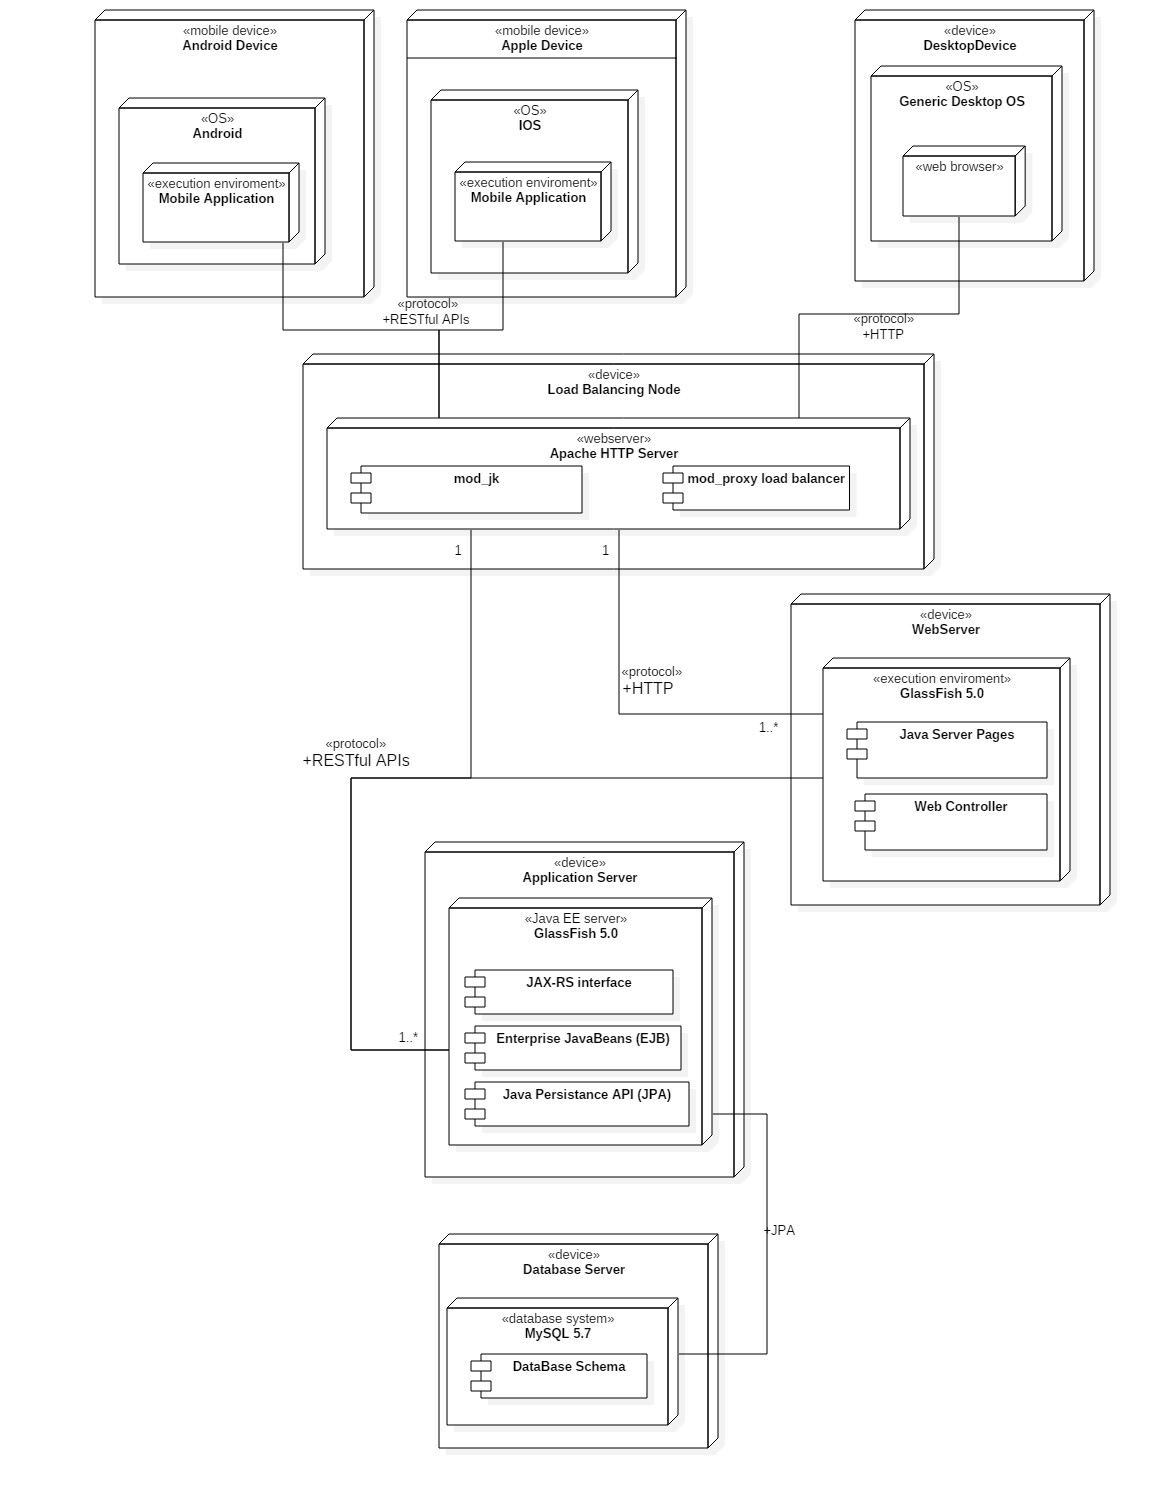
\includegraphics[scale=0.35]{DeploymentDiagram.png}
\end{center}
\caption{Deployment diagram}
\end{figure}

\subsection{Recommended Implementation Choices}
\label{subsect:Recommended Implementation Choices}
Here we provide a set of recommended implementation choices in order to actually develop the Travlendar+ system.
\begin{itemize}
	\item The \textbf{Database Server} may be implemented with MySQL 5.7 as Relational DBMS;
	
	\item The \textbf{Application Server} may be implemented using Java Enterprise Edition (JEE) 8, this choice could allow the developers to focus on the logic to be provided while being supported by reliable APIs and tools, in order to reduce the complexity of the development phase. Using JEE 8 the developers could also guarantee the main non-functional requirements, which are stated in RASD document. The specific JEE 8 choices can be:
	\begin{enumerate}[a)]
		\item GlassFish 5.0 as Application Server implementation;
		\item JPA (Java Persistence API) in order to interact with the database Database Server, in particular Entity Beans can be used to map the data;
		\item EJB (Enterprise Java Beans) in order to implement the business logic, in fact the components described in section \ref{subsect:Application Server} can be implemented as multiple Stateless Session Beans;
		\item JAX-RS in order to implement the interface used through the web with both mobile apps and the web server.
	\end{enumerate}
	
	\item The \textbf{WebServer} may be implemented using Tomcat 8 as HTTP web server implementation and JSP (JavaServer Pages) may be used to provide dynamically generated web pages;
	
	\item The \textbf{Load Balancing Node} may be implemented using an Apache HTTP Server;
	
	\item The \textbf{Android App} may be implemented using Java and XML programming languages;
	
	\item The \textbf{IOs App} may be implemented using Swift programming language.
\end{itemize}
\newpage
			
		\section{Runtime view}
		\label{sect:Runtime view}
			\subsection{Login}
			\noindent\makebox[\textwidth]{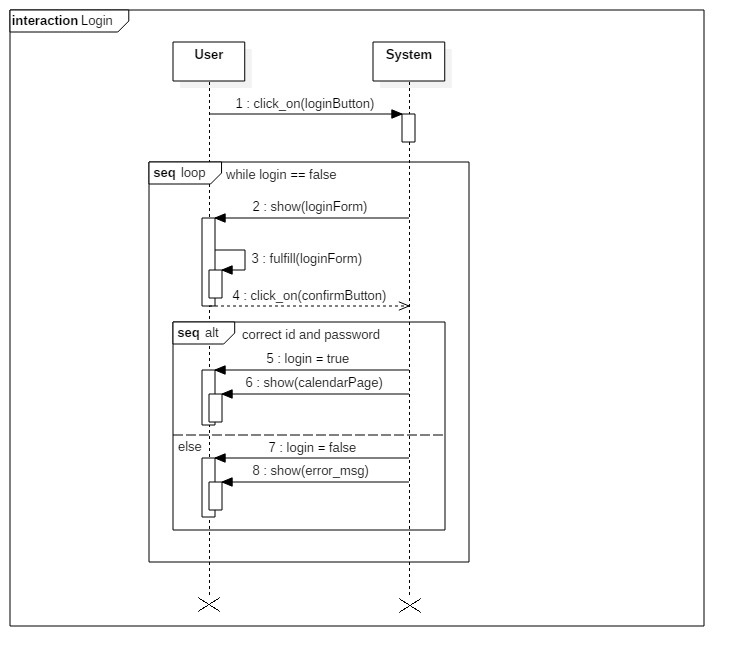
\includegraphics[width=\paperwidth,height=\paperheight,keepaspectratio]{sequence_diagrams/login.png}}
			The login operation is performed only the first time that the application is used. 
			The \textit{system} calculates a univocal code that is returned to the client and stored in the \textit{local DB}. In this way the client can be recognized for future operations. 
			The encryption function will be specified below in the document.
\subsection{Authentication functions for each operation}
		\noindent\makebox[\textwidth]{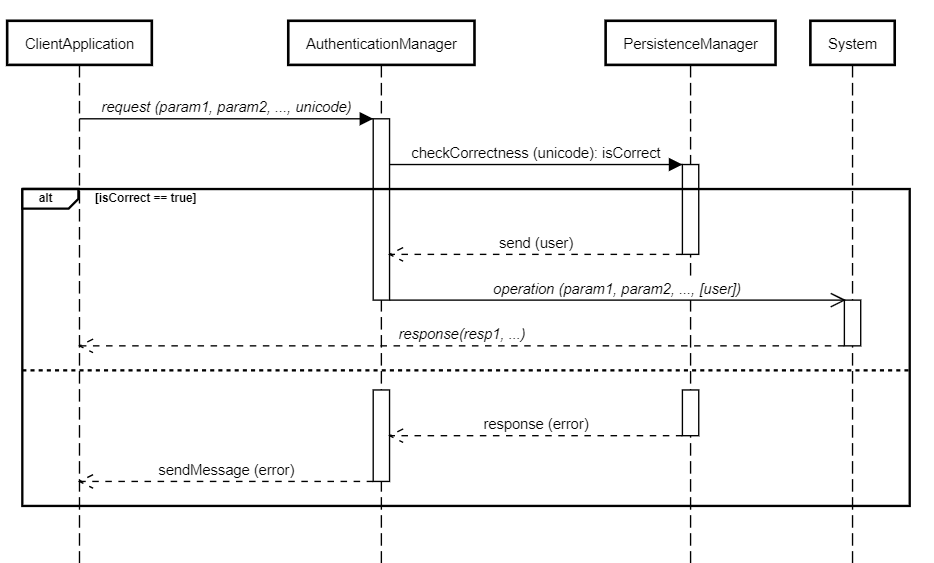
\includegraphics[width=\paperwidth,height=\paperheight,keepaspectratio]{sequence_diagrams/for_each_operation.png}}
		This is a model of how a generic request is taken into account by the system: the \textit{Client} sends the univocal code with the other parameters and the \textit{Authentication Manager} performs the check. 
		The \textit{Authentication Manager} forwards the request only if the univocal code is correctly recognized.
\subsection{Create event}
		\noindent\makebox[\textwidth]{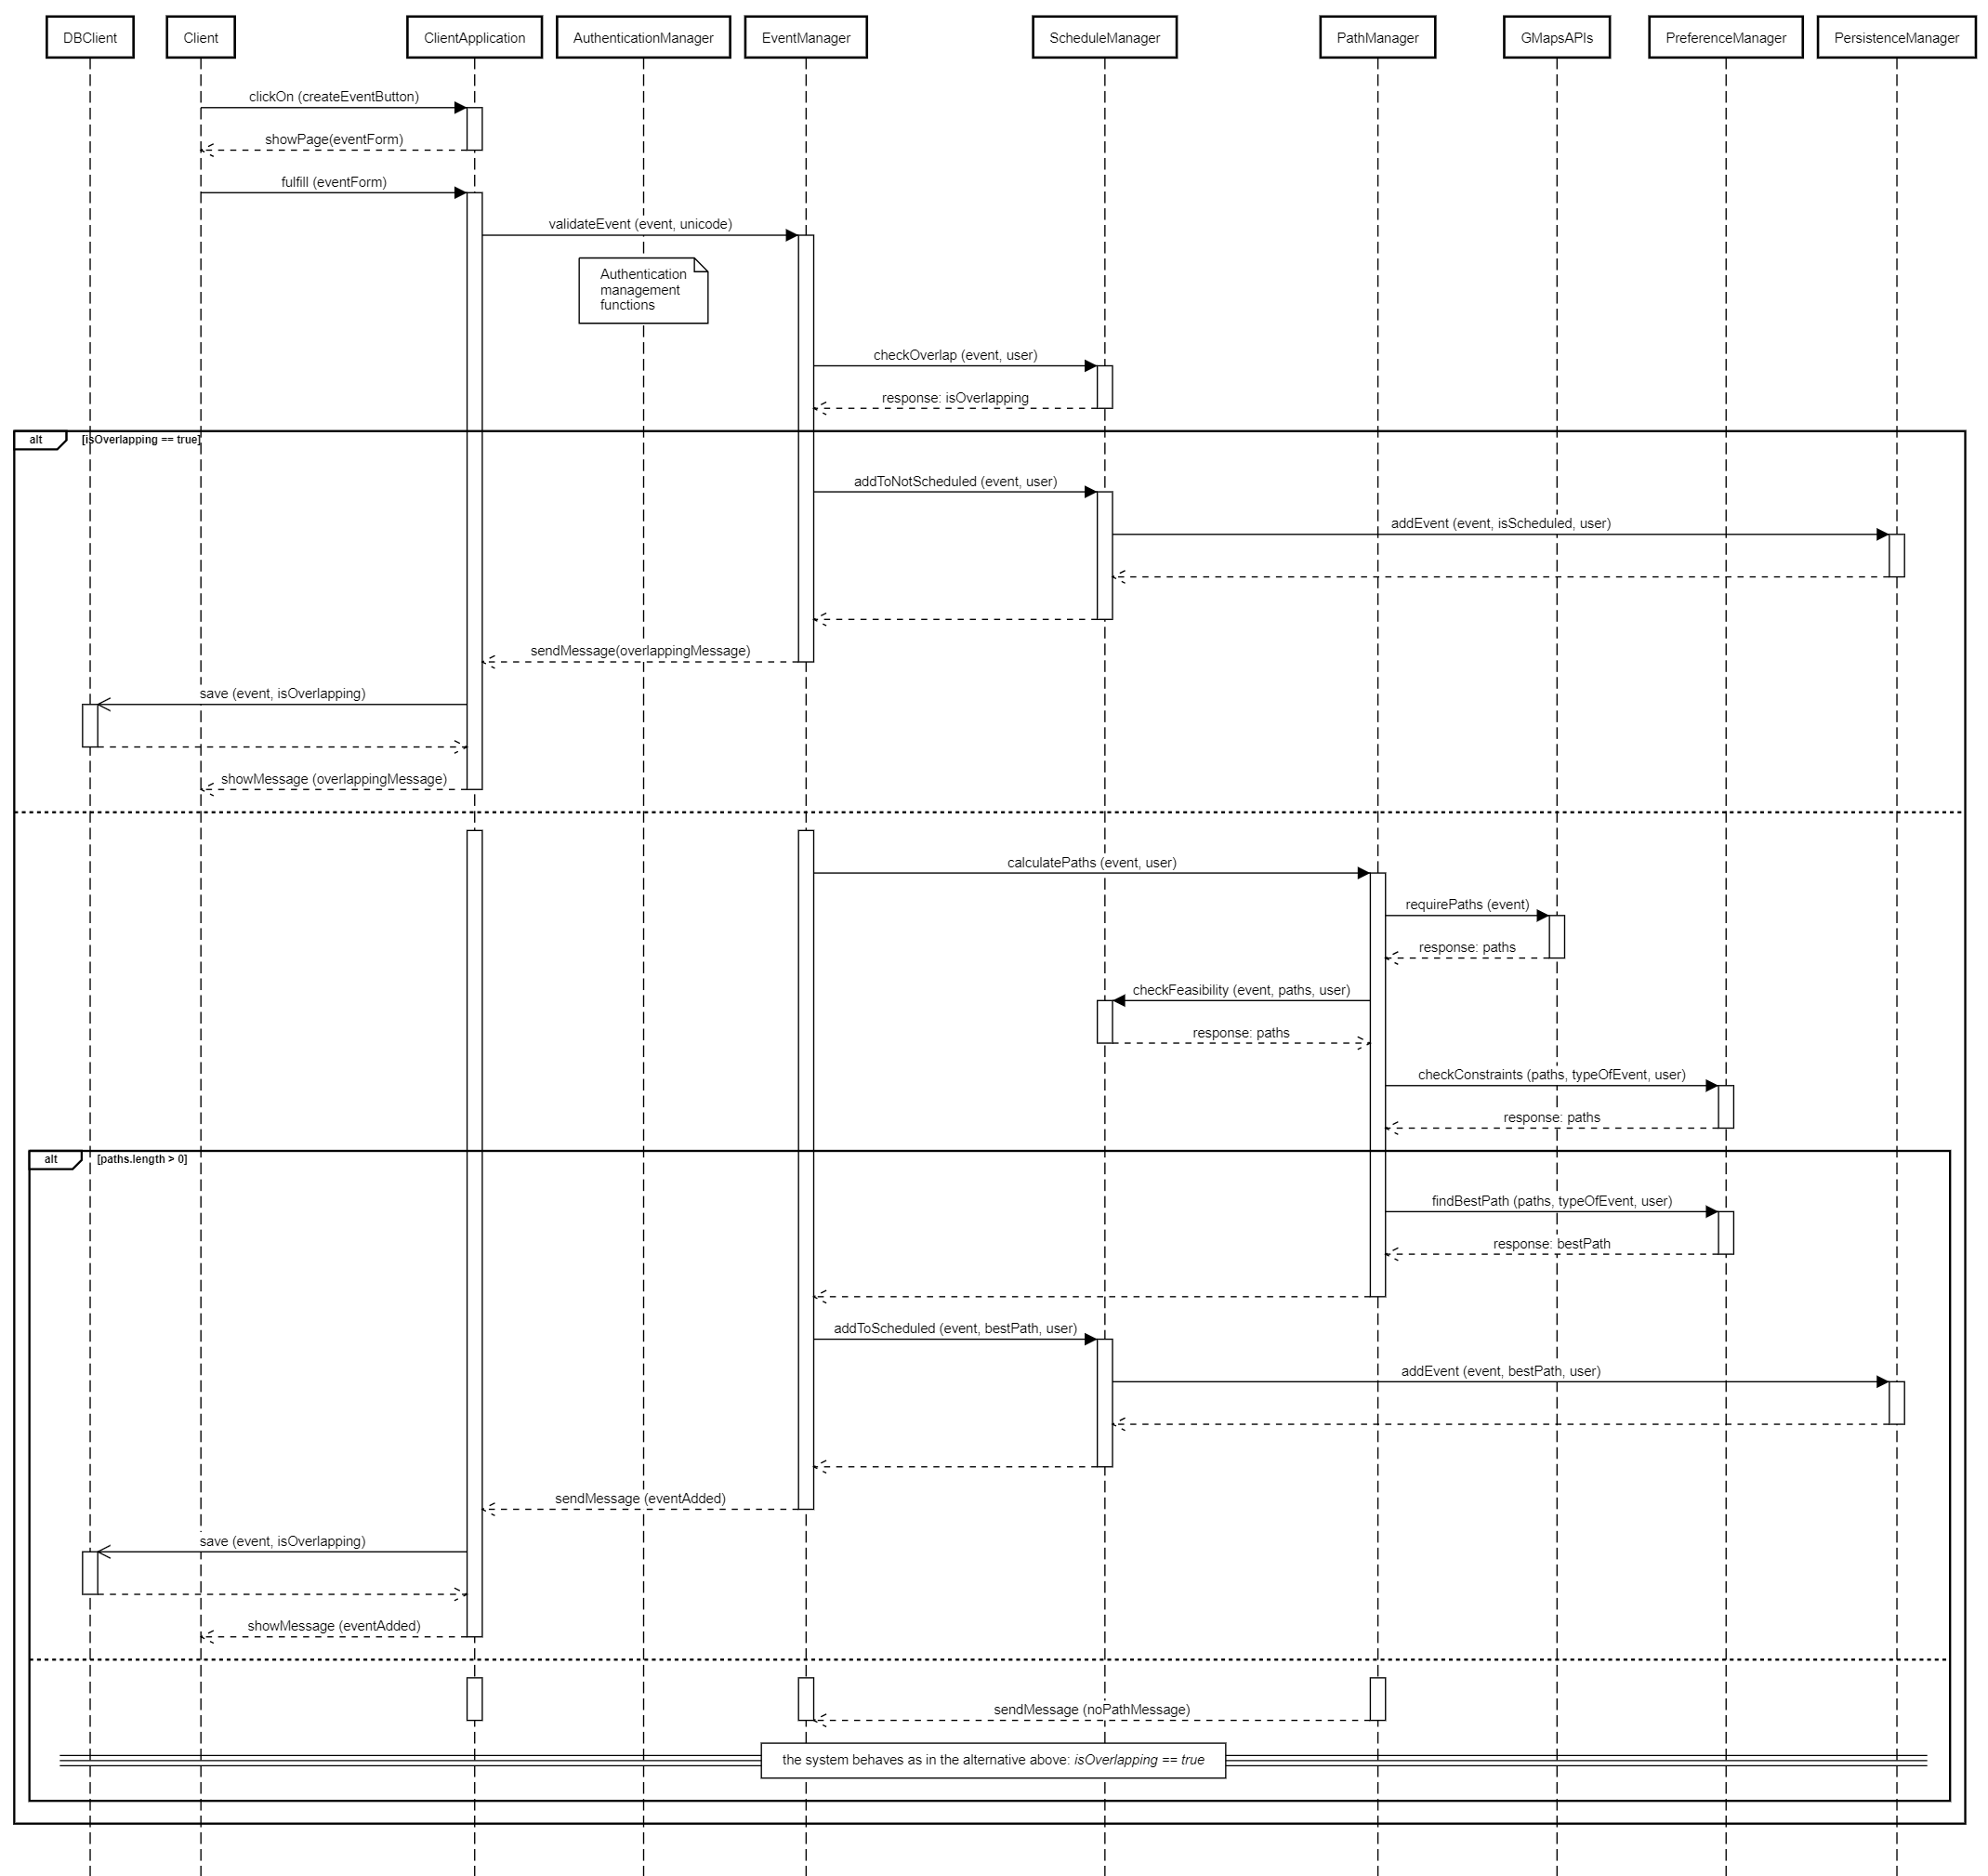
\includegraphics[width=\paperwidth,height=\paperheight,keepaspectratio]{sequence_diagrams/create_event.png}}
\subsection{Arrange trip}
		\noindent\makebox[\textwidth]{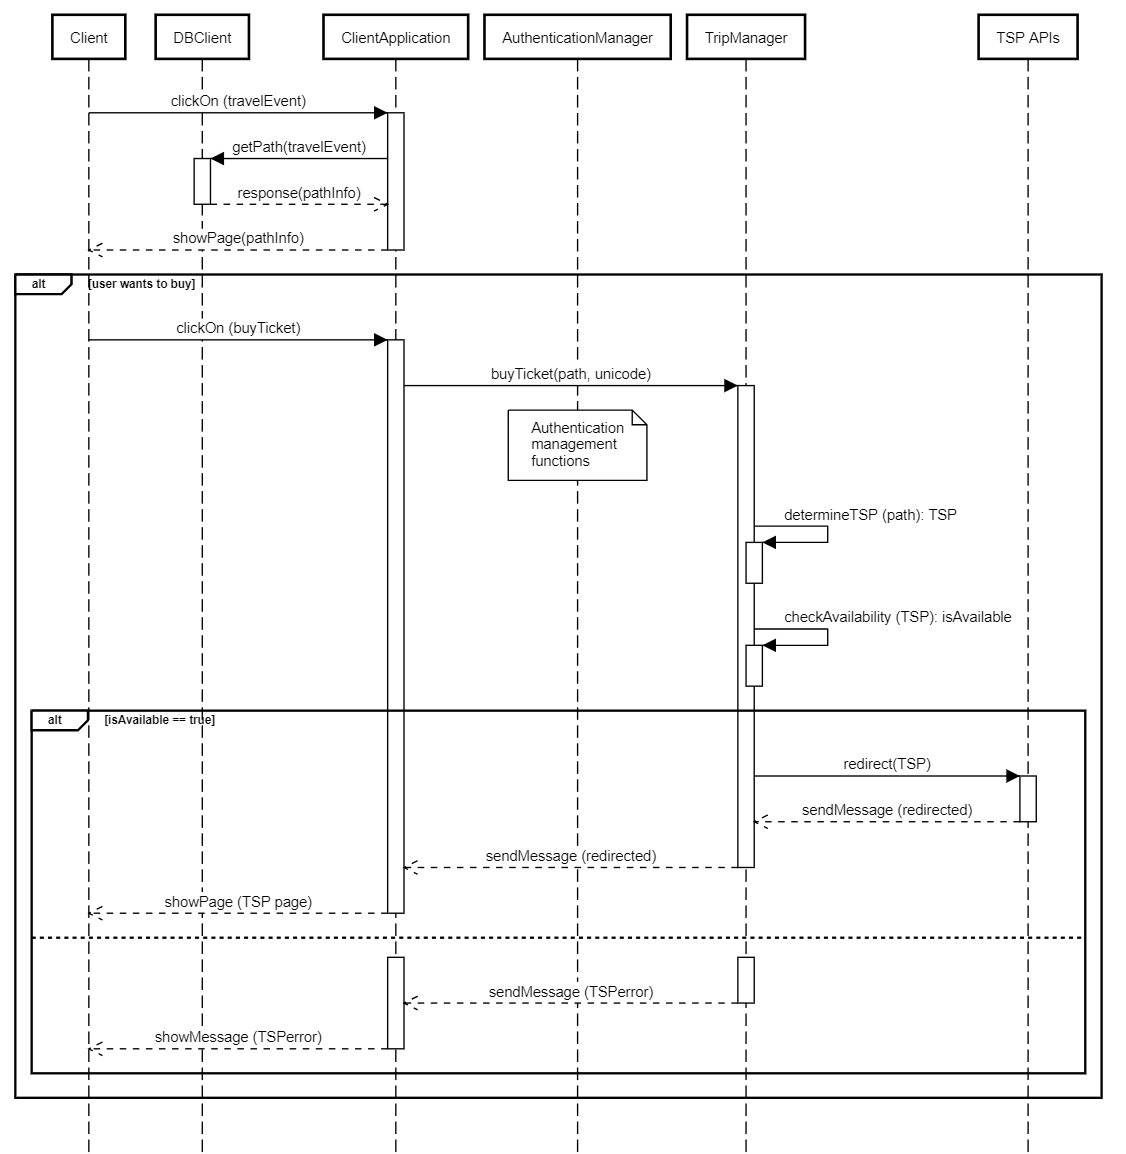
\includegraphics[width=\paperwidth,height=\paperheight,keepaspectratio]{sequence_diagrams/arrange_trip.png}}
\subsection{Obtain feasible paths}
		\noindent\makebox[\textwidth]{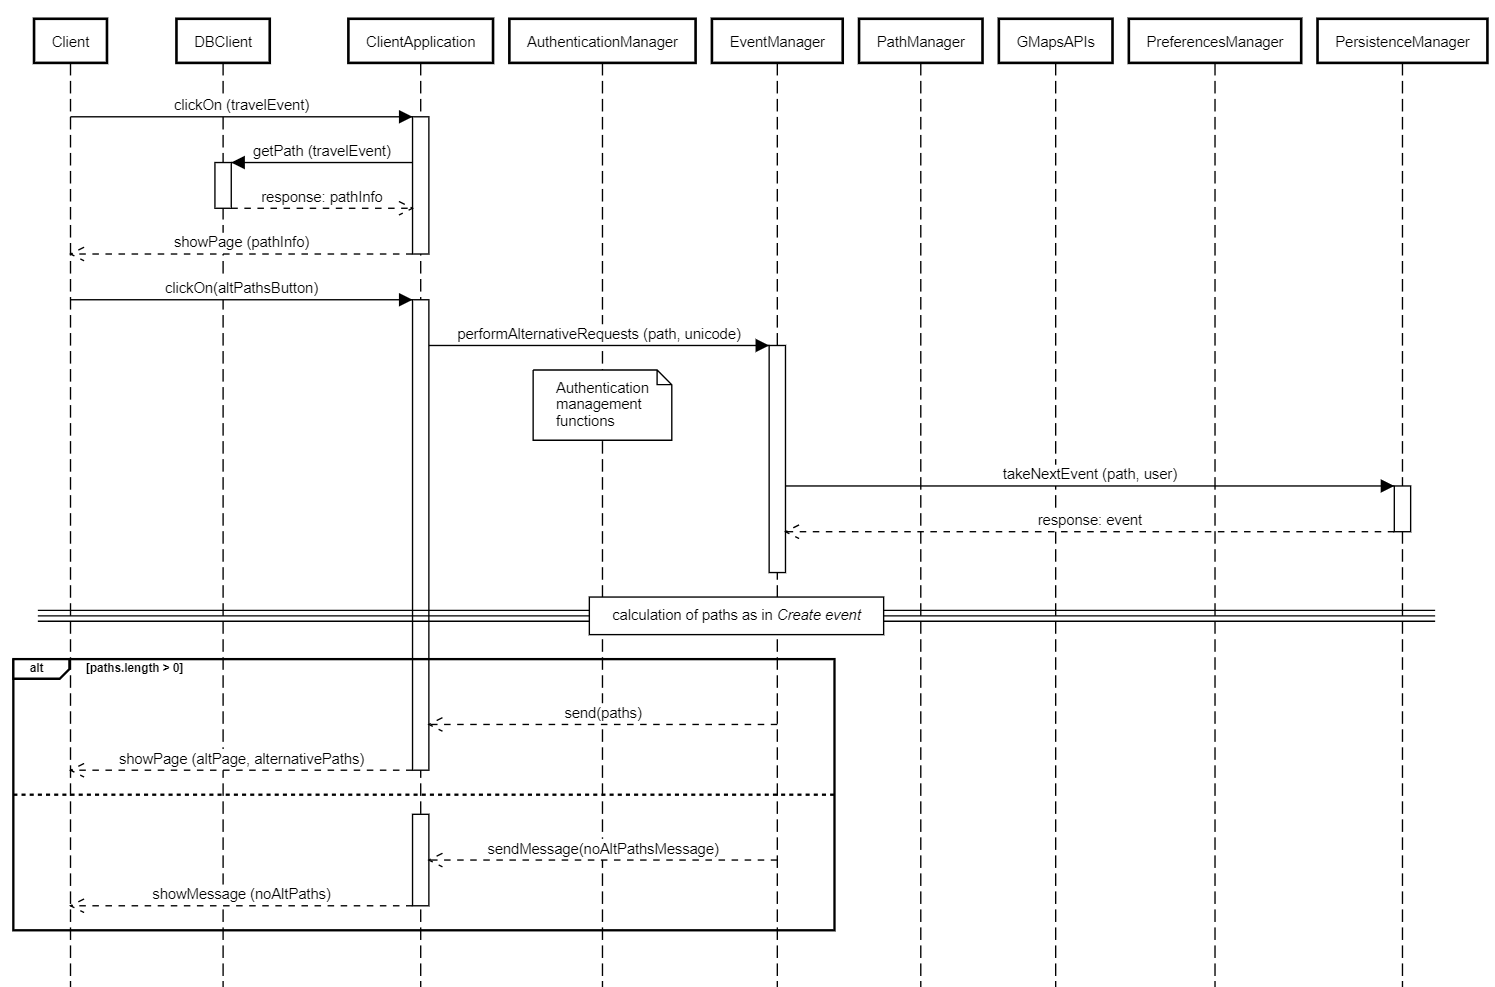
\includegraphics[width=\paperwidth,height=\paperheight,keepaspectratio]{sequence_diagrams/obtain_feasible_paths.png}}
		Only the best path is stored into \textit{local and server DBs}, so if a user wants to see alternative feasible paths, a new calculation of paths is needed. 
		The \textit{system} obtains the event related to the path and then calculates the feasible alternatives with the function of \textit{GMaps} and the checks on feasibility and constraints.
\subsection{Choose between overlapping events}
		\noindent\makebox[\textwidth]{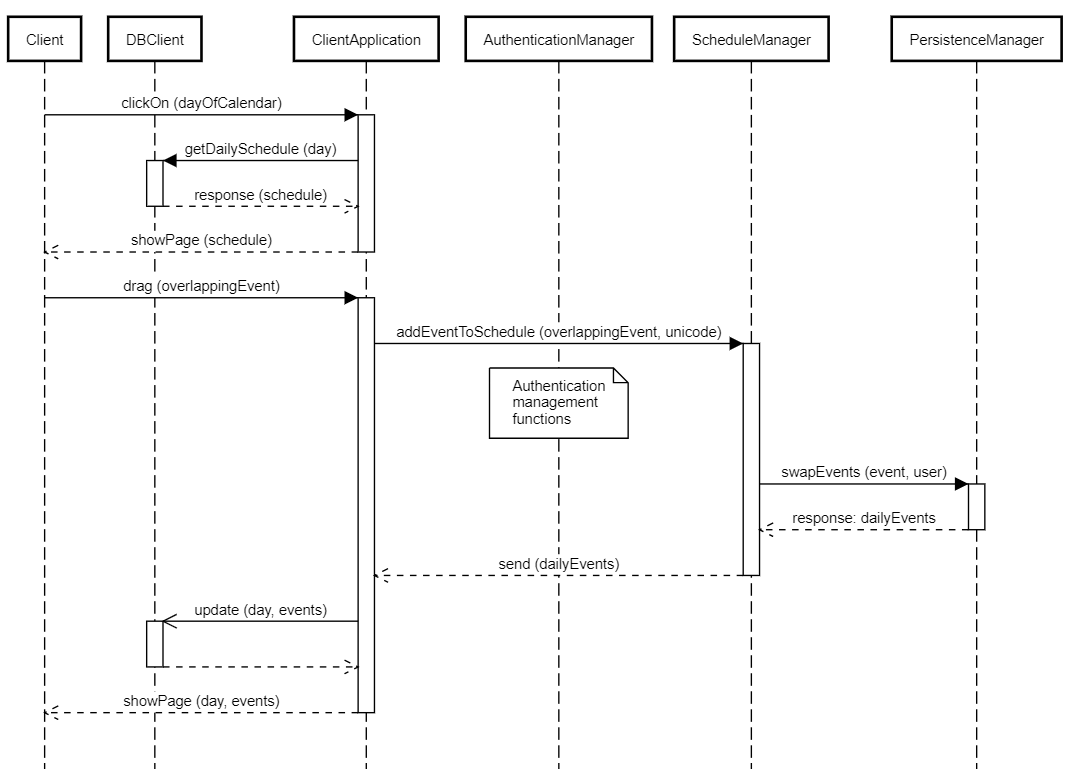
\includegraphics[width=\paperwidth,height=\paperheight,keepaspectratio]{sequence_diagrams/choose_between_overlapping_events.png}}
\subsection{Strike announcement}
		\noindent\makebox[\textwidth]{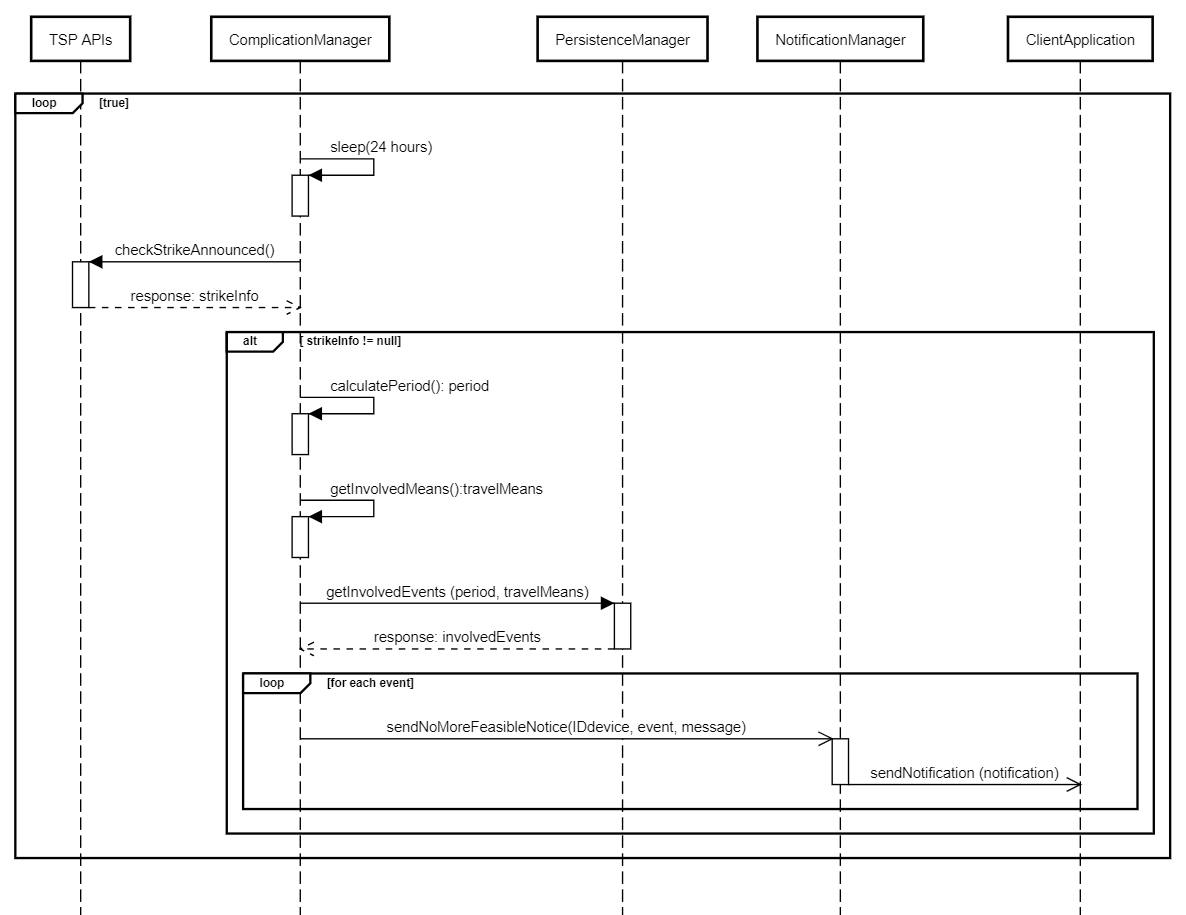
\includegraphics[width=\paperwidth,height=\paperheight,keepaspectratio]{sequence_diagrams/strike_announcement.png}}
		The \textit{Complication Manager} every day performs a list of operations, one of them is to check if a strike for the following days is announced. 
		In case of strike a notification is sent for each event stored in the \textit{database} that is involved: several notifications can be sent to the same user. 
		If the user opens the notification, \textit{obtain feasible paths} function, related to the involved event, is called.
			
		\section{Component interfaces}
		\label{sect:Component interfaces}
			\todo{TODO}
		
		\section{Selected architectural styles and patterns}
		\label{sect:Selected architectural styles and patterns}
			The following architectural styles and patterns have been used in order to ensure a well-formed and efficient architecture:

\subsection{Layered Architecture}
\label{subsect:Layered Architecture}
This architectural style allows to organize the system through abstraction levels and doing so it separates presentation, application logic and data management functionalities.\\ Furthermore, since each layer can be separately instantiated on a
different machine, this architecture guarantees great flexibility in terms of hardware configurations and simplifies the actual development of the system, cause all components can be implemented and tested separately.

\subsection{Client/Server}
\label{subsect:Client/Server}
Our application is strongly based on the client server paradigm and it's used at various levels:
\begin{itemize}
	\item the mobile application (client) makes requests to the Application Server (server) that replies to them;
	\item the web browsers (clients) communicates with the Web Server (server), which also acts as a client with respect to the Application Server.
	\item the Application Server acts as client when it interrogates the database Server or when it interacts with external APIs.
\end{itemize}

\subsection{Model-View-Controller}
\label{subsect:Model-View-Controller}
The proposed Travlendar+ system follows this pattern. This allows to separate the application into three communicating and interconnected abstract parts which fulfills different goals. In particular our system implements the so-called 'Apple MVC version', which always keeps the Controller between the model and the view interactions in order to guarantee security and access control. 

\subsection{Publish/Subscribe}
\label{subsect:Publish/Subscribe}
This architectural style is primarily used in the notification system. When a user mobile device logs into the system subscribes as listener and will receive notice of all possible problems involving the Travlendar+ user experience. This paradigm provides us great flexibility with respect to future expansions.

\subsection{Five Tier Architecture}
\label{subsect:Five Tier Architecture}
This Architectural style allows us to deploy the various physical components of our system on different devices, in order to separate responsibilities and also to introduce redundancy in order to improve the availability and reliability. 
\newpage

		
		\section{Other design decisions}
		\label{sect:Other design decisions}
			\subsection{Authentication}
\label{subsect:Authentication}
When the users log in into the system for the first time from a device the Application server will assign to that device an univocal Unicode code, so for further requests from that device (web browser or mobile application) the users can avoid to log in again. Every new request will include into the request payload that code, enabling the Application server to validate the request and to recognize the specific user that sent them. The univocal code will be generated by an internal algorithm in the AuthenticationManager (explained in section \ref{sect: Univocal code}). The AuthenticationManager will check every time the consistency of the univocal code and it will also check if it comes from the same device it is associated to.\\
If a log in is performed from an already registered device but it comes from a different Travlendar+ account the previous univocal code associated to that device will be deleted, and the previous user will have to log in again with his previous account.

\subsection{Encryption}
\label{subsect:Encryption}
The encryption is used only to send password from the client to the server. For the other operations, in fact, the client exploits the univocal code described below in order to authenticate itself. This code is used in combination with the ID of the device that send the request, so encryption for the univocal code is not necessary.\\
To encrypt the password is suitable a \textit{public key algorithm} because it allows to send the string in a secure and easy way on internet and the size of data to encrypt is small.\\
A public key algorithm uses a pair of keys: a \textit{public key} distributed to the clients and a \textit{private key} known only by the server. The client encrypts the password with the public key and send it to the server; the server is the only one able to decrypt the message thanks to the private key.\\
The encryption in the system is implemented according to the \textit{RSA algorithm}.

\subsection{Notifications}
\label{subsect: Notifications}
In order to send notifications to the mobile devices our system will memorize the Identifiers of the user devices, and when a notification is to be sent the Application Server will interact with the interfaces offered by GCM (Google Cloud Messaging) in order to actually forward them to the user devices. We choose to use GCM services cause they handle all aspects of queueing of messages and delivery to client applications running on different target devices, and cause it is completely free.

\subsection{Local database update}
\label{subsect:Local database update}
When the application performs an operation that require a connection, both online and local database are updated. The user however can perform an operation on a different mobile device or with the browser, in these cases the local database of the application must be updated.\\
When the online database is modified, the system sends a notification to all the mobile devices related to the user whose local database isn't updated yet. The notification mechanism works as specified in section \ref{subsect: Notifications}. Only changes made after the last writing operation on local database are sent from server to local DB, in order to update it.

\subsection{Periodic events}
Once a day, an internal module is run to check that every periodical event inserted by a user is covered for a year, e.g. if an event like "Friday lunch with parents" with a weekly periodicity is created on 2018/01/05, on 2018/01/12 the module will create a new event on 2019/01/12.

			
	\chapter{ALGORITHM DESIGN}
	\label{ch:ALGORITHM DESIGN}
		In this section we will give an overall description of the main algorithms required in order enable Travlendar+ system to work as intended and to satisfy both functional and non functional requirements.

\section{Path calculation}
\label{sect:Path calculation}
	In order to compute optimal paths that include also sharing vehicles, not included into the set of possible travel means offered by \textit{Google Map APIs}, the system will have to implement some additional logic. We will handle the sharing vehicles option as an additional possible public travel mean, for example an user could want to take a bike in sharing instead of taking the subway.\\
The algorithm that implements this functionality will follow the behavior explained in the pseudo-code below:
\begin{figure}[H]
\begin{center}
		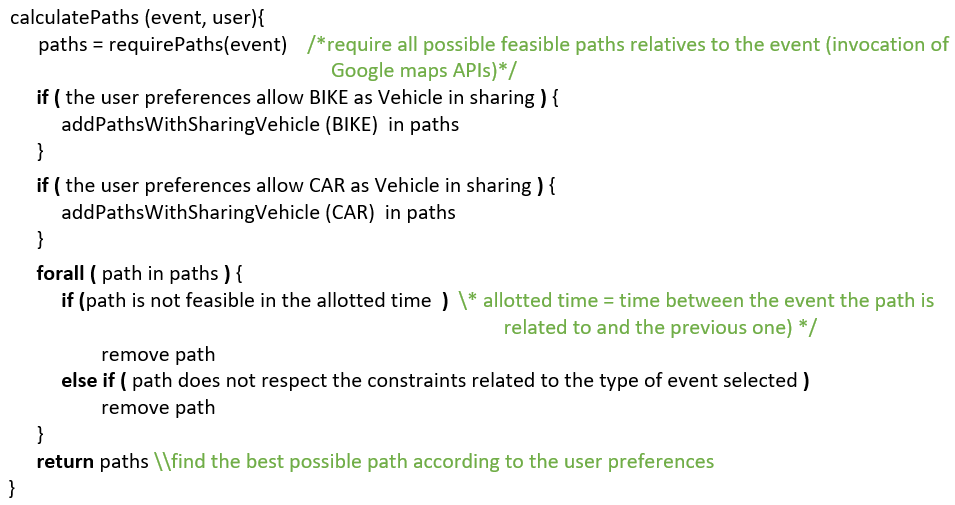
\includegraphics[width=\textwidth]{algorithms/calculate_paths.png}
\end{center}
\end{figure}
\noindent The addPathsWithSharingVehicle method is explained below:
\begin{figure}[H]
\begin{center}
		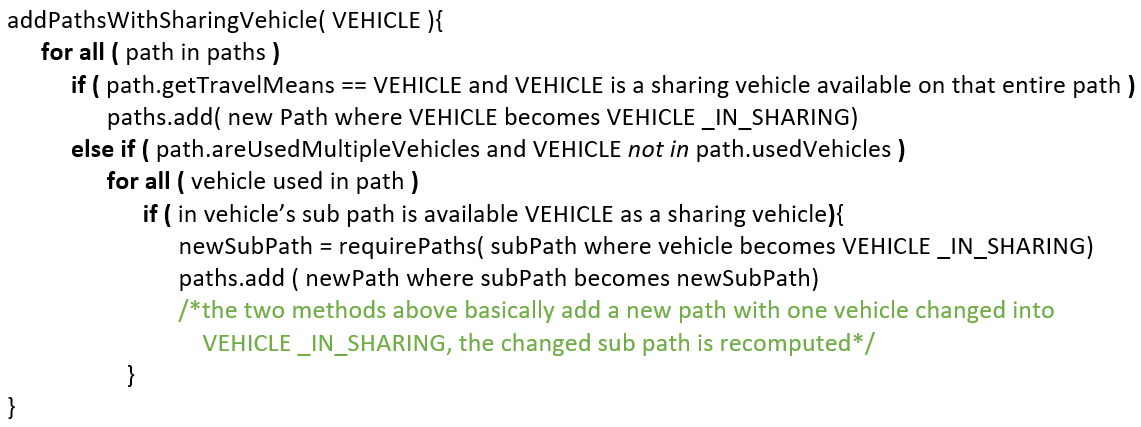
\includegraphics[width=\textwidth]{algorithms/sharing_method.png}
		
\end{center}
\end{figure}


\section{Univocal code}
\label{sect: Univocal code}
	In the registration process the username and the password (sended with the encryption algorithm specified above) are written in the database.\\
Log in operation is required in order to use the functionalities of the system.
\\\\
When login happens the user inserts username and they are sended to the system; the system also obtains the ID device exploiting a GCM's function. In the DB several IDdevices can be associated to the same user, there is a field that marks the ID as mobile (related to phones and tablets) or browser (related to PCs). Browser IDs are deleted periodically. 
\\\\
The system behaves as specified in the flowchart according to the situation:
\begin{itemize}
\item first access: device is not present in the database;
\item login with different device: device is in the database, but it is associated to a different user;
\item login with the same device (not for the first time): a new univocal code is calculated and it will be update on the database.
\end{itemize}
The univocal code is a randomly generated string concatenated to the username (unique). The random string is calculated with the Current Unix Timestamp.
\\\\
The univocal code is sent to the device (a parameter that will be stored locally in the case of a mobile application, a cookie in the case of a browser) and will be used for every interaction with the system: in this way happens the identification of the user. For each request the system takes the univocal code received and the ID of the device and checks in the database if they are related.
\\
\begin{figure}
	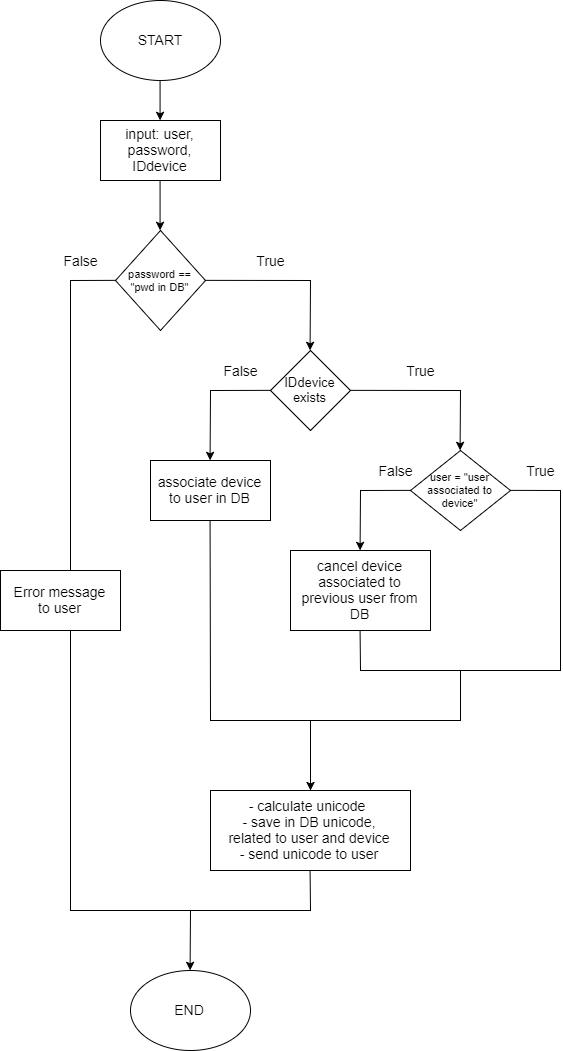
\includegraphics[scale=0.6]{algorithms/unicode_fc.png}
	\centering
	\caption{What happens during the login phase}
\end{figure}


\section{Swap events in the schedule}
\label{sect: Swap events in the schedule}
	The purpose of this algorithm is to check and manage the schedule when an overlapping event is forced into it, maintaining thus a feasible list of scheduled events. \\ \\
To explain it we will use the following terms: 
\begin{itemize}
	\item \textit{ForcedEvent}: The event that is going to be put into the schedule;
	\item \textit{ScheduledEvent}: An event that will be removed from the schedule as a consequence of the ForcedEvent insertion;
	\item \textit{ScheduleList}: A list containing all the scheduled events for a specific day;
	\item \textit{OverlappingList}: A list containing all the overlapping events for a specific day.
\end{itemize}
\newpage
\noindent The algorithm works in this way:
\begin{enumerate}
	\item Checks if there are ScheduledEvents with: \\ \textit{startingTime(ScheduledEvent) \textless startingTime(ForcedEvent) \textless endingTime(ScheduledEvent)} \\ or \\ \textit{startingTime(ScheduledEvent) \textless endingTime(ForcedEvent) \textless endingTime(ScheduledEvent)} \\
or \\ \textit{startingTime(ForcedEvent) \textless startingTime(ScheduledEvent) AND \\endingTime(ScheduledEvent) \textless endingTime(ForcedEvent)}. \\
	If the condition results True for one or more scheduled events, it removes them from the schedule and puts them in the overlapping list;
	\item Computes the travel of ForcedEvent, depending on the previousLocation inserted or, if a previous starting location for the travel is not defined, on the location of the previous ScheduledEvent;
	\item If the travel used to reach the ForcedEvent requires a departure time that is less than the previous ScheduledEvent ending time, the previous ScheduledEvent is removed from the ScheduleList and added to the OverlappingList;
	\item Repeats 2 and 3 until a ScheduledEvent considered is still feasible after the insertion of the ForcedEvent;
	\item Recomputes the travel of the ScheduledEvent that follows ForcedEvent. If that ScheduledEvent's location is not reachable in time for its starting time anymore, this ScheduledEvent is removed from the ScheduleList and added to the OverlappingList;
	\item Repeats 5 until the ScheduledEvent following ForcedEvent in the ScheduleList is still a feasible one after the recomputation of its travel;
	\item ForcedEvent has been successfully inserted in the schedule.
\end{enumerate}

\section{Flexible breaks}
\label{sect: Flexible breaks}
	The purpose of this algorithm is to check if a flexible break inserted is respected by the events present in the schedule. \\ \\
To explain it we will use the following terms: 
\begin{itemize}
	\item \textit{BreakList}: a list containing all the events that overlap, even partially, with the flexible break time slot;
\end{itemize}
The algorithm works in this way:
\begin{enumerate}
	\item Puts in BreakList all the scheduled events that take place during the allotted break time slot, even if partially;
	\item Checks if at least one of the spare time slots between an event of BreakList and the following one (including travels) is larger enough to include the break event;
\end{enumerate}	
SPECIAL CASE: if only one event is present in BreakList, the algorithm must check that the remaining spare time in the slot is larger enough to allocate the break event.

\section{Periodical events}
\label{sect: Periodical events}
	The purpose of this algorithm is to manage the creation of periodical events. \\ \\
The algorithm works in this way: when a periodical event is inserted, a number of events is generated in order to cover a span of one year, e.g. if an event like "Friday lunch with parents" with a weekly periodicity is created, 52 different events will be created.
To better understand the reasoning behind this, take a look at section \ref{sect:Other design decisions}.


			
	\chapter{USER INTERFACE DESIGN}
	\label{ch:USER INTERFACE DESIGN}
		\todo{TODO}
	
	\chapter{REQUIREMENTS TRACEABILITY}
	\label{ch:REQUIREMENTS TRACEABILITY}
		\begin{center}
	\begin{longtable}{ | p{0.3\textwidth} | p{0.7\textwidth} | }
		\hline
		\textbf{Component} & \textbf{Requirement}\\
		\hline
		Authentication Manager & \textbf{[R1]} the system checks if the e-mail inserted is real;\\
		& \textbf{[R2]} a user cannot sign up with the same e-mail twice;\\
		& \textbf{[R3]} the e-mail and password inserted must be correct;\\
		& \textbf{[R4]} incorrect credentials prevent the user from logging in;\\
		& \textbf{[R38]} a user must be logged.\\
		\hline
		Path Manager & \textbf{[R10]} every travel path proposed must be feasible in the available time (the interval between two consecutive events);\\
		& \textbf{[R11]} if the travel involves two or more travel means, the starting location of the first proposed travel path and the ending location of the last proposed travel path must coincide respectively with the starting location and the ending location of the whole planned travel;\\
		& \textbf{[R12]} the system does not consider paths that violate constraints on travel means defined by the user;\\
		& \textbf{[R13]} the system checks user preferences to decide which feasible travel path is the best;\\
		& \textbf{[R15]} appropriate travel means must be suggested according to the type of event that they are related to; \\
		& \textbf{[R18]} the system must show to the user all possibilities to reach a location in according with the requirements of [G4];\\
		& \textbf{[R19]} alternative feasible travel paths must not generate overlappings with other events of the schedule;\\
		& \textbf{[R25]} the system does not consider solutions that violate constraints;\\
		& \textbf{[R27]} the system does not consider solutions that include deactivated travel means;\\
		& \textbf{[R28]} for each travel path, the system estimates its carbon footprint produced;\\
		& \textbf{[R35]} the system provides information about time of departure and arrival of the proposed travels;\\
		& \textbf{[R37]} the system provides information about travel time with shared vehicles.\\
		\hline
		Event Manager & \textbf{[R5]} a user must specify all mandatory fields to add the new event;\\
		& \textbf{[R6]} the system reserves the specified time-slot for the event;\\
		& \textbf{[R7]} the system warns the user if the inserted event overlaps with an already existing one;\\
		& \textbf{[R8]} if the ending time of an event is not specified, the systems considers as ending time the hour of departure for the successive event;\\
		& \textbf{[R9]} when an event is inserted after an event without a specified ending time, the ending time  of the first event is anticipated as stated in [R8];\\
		& \textbf{[R29]} the system allows the user to specify a flexible interval and a minimum amount of time to schedule a break;\\
		\hline
		Schedule Manager & \textbf{[R6]} the system reserves the specified time-slot for the event;\\
		& \textbf{[R7]} the system warns the user if the inserted event overlaps with an already existing one;\\
		& \textbf{[R8]} if the ending time of an event is not specified, the systems considers as ending time the hour of departure for the successive event;\\
		& \textbf{[R9]} when an event is inserted after an event without a specified ending time, the ending time  of the first event is anticipated as stated in [R8];\\
		& \textbf{[R14]} the system warns the user if it is not possible to arrive at an event location before its starting time;\\
		& \textbf{[R19]} alternative feasible travel paths must not generate overlappings with other events of the schedule;\\
		& \textbf{[R20]} the combination of the travel paths proposed for the day must be feasible in the allotted time;\\
		& \textbf{[R21]} if there are multiple events at the same time the system will propose in the schedule only the first event added;\\
		& \textbf{[R22]} if the user forces into the schedule an event that overlaps with events already present in the schedule, these are removed from the schedule;\\
		& \textbf{[R30]} if there is enough time for a break, the system reserves it within the specified flexible interval;\\
		& \textbf{[R31]} if there is not enough time into the flexible interval specified, a warning is thrown.\\
		\hline
		Preference Manager & \textbf{[R12]} the system does not consider paths that violate constraints on travel means defined by the user;\\
		& \textbf{[R13]} the system checks user preferences to decide which feasible travel path is the best;\\
		& \textbf{[R15]} appropriate travel means must be suggested according to the type of event that they are related to; \\
		& \textbf{[R23]} the system requires minimum and maximum length allowed for a path to impose a constraint on a travel mean;\\
		& \textbf{[R24]} the system requires an interval of time allowed to impose a constraint on a travel mean;\\
		& \textbf{[R25]} the system does not consider solutions that violate constraints;\\
		& \textbf{[R26]} the system allows the user to specify one or more travel means that cannot be used;\\
		& \textbf{[R27]} the system does not consider solutions that include deactivated travel means.\\
		\hline		
		Trip Manager & \textbf{[R32]} the system allows the user to specify all the ticket he already owns;\\
		& \textbf{[R33]} the system shows to the user if he already holds a ticket for a proposed travel;\\
		& \textbf{[R34]} the system allows the user to buy public transportation tickets according to proposed travels;\\
		& \textbf{[R36]} the system shows to the user where sharing vehicles are located.\\
		\hline
		Complication manager & \textbf{[R16]} if a strike occurs, the system will not consider travel means involved in it;\\
		& \textbf{[R17]} if the weather forecasts rain or other adverse conditions, the system will not consider paths involving the bicycle.\\
		\hline
		Notification Manager & \textbf{[R14]} the system warns the user if it is not possible to arrive at an event location before its starting time;\\
		& \textbf{[R31]} if there is not enough time into the flexible interval specified, a warning is thrown.\\
		\hline
		
		\caption{Application server components}
	\end{longtable}
\end{center}
The \textit{Notification Manager} is used to satisfy the above requirements and also to warn the user when a strike is announced or when the weather forecasts for the following days are adverse.\\\\
The \textit{Persistence Manager} allows the system to interact with database and helps the system to keep up-to-date the local database. In order to perform any operation concerning the data, the system queries and updates the server database. Information about events and paths are stored also in the local database of mobile phones: in this way the mobile app doesn't require a connection to show user's schedules. 
			
	\chapter{IMPLEMENTATION, INTEGRATION AND TEST PLAN}
	\label{ch:IMPLEMENTATION, INTEGRATION AND TEST PLAN}
		\section{Implementation Plan}
In this section we explain the order in which we plan to implement the subcomponents of the Travlendar+ system.
The main criteria we've adopted is to implement first a core of functionalities that we consider to be essential for engaging an initial user base, then we will proceed to insert new and nice-to-have features but that are not mandatory in a first release.\\
These are the main steps of the implementations we want to follow, in order to reach Travlendar+ full operativity on\begin{large}
\textbf{server side}:
\end{large}
\begin{enumerate}
\item \textit{CalendarManager} (\textit{PathManager}, \textit{EventManager}, \textit{ScheduleManager}, but not \textit{PreferenceManager}), \textit{PersistenceManager} and \textit{AuthenticationManager} are the core of our system and so they are the first to be implemented among with their subcomponents. In particular in this phase the user will not be able to edit his travels but he can only visualize the proposed ones;
\item \textit{PreferenceManager} will be inserted at a later time, in order to filter the user paths. Doing so there will be added functionalities that allow the user to edit and choose the travels he prefers from the feasible ones, which have been proposed to him;
\item \textit{ComplicationManager} will be added together with the \textit{NotificationManager} in order to allow the system to discover if a users travel is no more feasible and notify him.
\item \textit{TripManager} will be the last module to be implemented, allowing the user to arrange his trips.
\end{enumerate}
Of course at each implementation phase some data structures are to be added in the database (through the \textit{PersistenceManager}) to proper support the new functionalities.\\ \\
\noindent
These are the main steps of the implementations we want to follow to reach Travlendar+ full operativity on\begin{large}
\textbf{client side}:
\end{large}
\begin{enumerate}
\item Android App is to be developed first, proper updated will be performed when a new functionality is added on server-side, but the first application version is to be released together with the Application Server core functionality release;
\item IOS App will be developed in a second phase: when the Android application is completed (first release). The workforce dedicated to his development will be moved on this task but Android App's support will be taken care of nonetheless;
\item When both IOS and Android applications are released we will proceed to develop the web server that will allow the users to use Travlendar+ from any web browser.
\end{enumerate}

\section{Integration Entry Criteria}
Before starting the integration and testing phase there are a number of conditions that have to be met:
\begin{itemize}
\item \textbf{Documents:} this document (DD) and RASD have to be completed;
\item \textbf{Proper Documentation:} Every method and class, before being tested must be provided with proper documentation and/or comments in order to ease the testing process and also make easier the reuse of the classes and their methods;
\item \textbf{Code Inspection and Analysis:} At least one method, either code inspection or automated data flow analysis, have to be performed on the modules and classes before we proceed to the integration and test phase that involves them;
\item \textbf{Starting Condition:} The integration process can start only if the component involved offers at least 75\% of their functionalities to-be-implemented, this means that this phase can start in parallel with the completion of that component, and not that the testing phase can end with some functionalities still to be implemented; 
\item \textbf{Unit tests:} Before starting the integration of one component, it must be tested through proper unity tests, in order to guaranteed a correct behavior of his internal mechanisms.
\end{itemize}
\section{Elements to be integrated}
Basically all the system components, specified in section \ref{sect:Component view}, need to be integrated together; here we specify in detail all the integration that need to be performed.\\
On Application Server side:
\begin{itemize}
	\item \textit{ScheduleManager}, \textit{EventManager} and \textit{PathManager} needs to be integrated together;
	\item \textit{PreferenceManager} needs to be integrated with \textit{PathManager} (NB: doing that the entire \textit{CalendarManager} subsystem will be integrated);
	\item \textit{TripManager} needs to be integrated with \textit{ComplicationManager};
	\item \textit{ComplicationManager} needs to be integrated with both \textit{NotificationManager} and \textit{TripManager};
	\item PersistenceManager needs to be integrated with our DBMS;
	\item All the components that rely on \textit{RESTful APIs} to implement the interaction with the clients need to be integrated and tested;
	\item Basically all the application server components rely on \textit{PersistenceManager} and therefore they need to be integrated with it, the same consideration is valid for the \textit{AuthenticationManager} (except for the \textit{NotificationManager} that does not interact with it).
\end{itemize}
On client side (App Mobile):
\begin{itemize}
	\item \textit{DBManager} needs to be integrated with the \textit{LocalDatabase};
	\item \textit{ApplicationController}, \textit{GUIManager} and \textit{DBManager} needs to be integrated together.
\end{itemize}
On web server side \textit{WebController} and \textit{JavaServerPages} needs to be integrated together.
All the interactions that single components have with external services APIs have to be tested and their correctness have to be guaranteed before integrate and test phase involving those components begins.

\section{Integration Testing Strategy}
The integration testing strategy we will adopt will be defined by a mix of two strategies and according to the  implementation plan. \\
The first strategy we are going to use is based on a \textbf{bottom-up approach}. This choice will allow us to start from the less-dependent components and then climb the "uses" hierarchy, through the use of proper drivers. The bottom-up approach will enable us to follow the implementation plan, that follow a similar approach. Doing so we will improve the efficiency and the parallelism of the development process. \newline
The bottom-up strategy will be mixed with a \textbf{critical-module-first approach}, in order to start the integration and testing of the most critical modules of our system, those contained in \textit{CalendarManager}. We've considered also this second strategy in order to avoid issues related to core components of our system and threats to the correct behavior of our system, especially to guarantee the absence of failures or bugs that could prevent the users to correctly take advantage of our platform and its functionalities.

\section{Sequence of Components integration}
The following subsections aim to describe the order in which Travlendar+ will have to be integrated and tested. We will use as notation an arrow going from component A to component B means that component A is necessary to component B and so it must have been already implemented before performing the integration.

\subsection{Software integration Sequence}
Since our system rely on some external systems and interact with theirs external interfaces (APIs) we will assume that those system are already proper tested. In order to test the interaction with all the external systems, we'll use first proper stubs that emulate their behavior and then we'll use the real external system; this is to be done in order to avoid that test are slowed, that connectivity issues cause test to fail and that during the tests we hit some APIs rate limits (for example with Google Maps APIs).

\subsubsection{PersistenceManager}
The first component to be integrated is the \textit{PersistenceManager}, since all other modules that have to access the data need this module in order to work properly. \textit{PersistenceManager} is to be integrated with the DBMS. To do some driver will be needed in order to perform queries, data insertion and deletion; A test database have to be introduced to perform such tests.
\begin{figure}[H]
	\begin{center}
		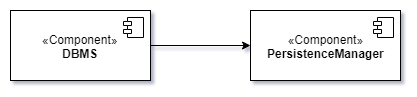
\includegraphics[scale=0.6]{implementation_and_testing/persistence.png}
	\end{center}
	\caption{I\&T - PersistenceManager}
\end{figure}

\subsubsection{AuthenticationManager}
Nearly every core-component require the \textit{AuthenticationManager} to work properly. It is to be integrated with the \textit{PersistenceManager}. A driver will simulate every possible authentication request.
\begin{figure}[H]
	\begin{center}
		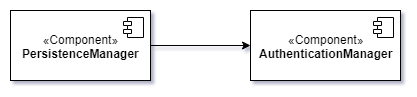
\includegraphics[scale=0.6]{implementation_and_testing/authentication.png}
	\end{center}
	\caption{I\&T - AuthenticationManager}
\end{figure}

\subsubsection{CalendarManager}
The \textit{CalendarManager}'s components interact all with \textit{AuthenticationManager} and \textit{PersistenceManager}, and so each component will be integrated with them. Since all \textit{CalendarManager}'s components offers an external interface to be exposed as RESTful services, a driver for each one of this components will be needed.\\
The \textit{CalendarManager}'s components are strictly correlated and so, in order to minimize the number of drivers and stubs, their integration order will be the following:\\
\indent 1. \textit{ScheduleManager} and \textit{PreferenceManager} are to be integrated with \textit{AuthenticationManager} and \textit{PersistenceManager}.
\begin{figure}[H]
	\begin{center}
		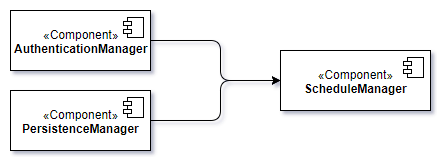
\includegraphics[scale=0.6]{implementation_and_testing/calendar_manager/schedule.png}
	\end{center}
	\caption{I\&T - ScheduleManager}
\end{figure}
\begin{figure}[H]
	\begin{center}
		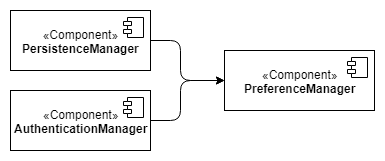
\includegraphics[scale=0.6]{implementation_and_testing/calendar_manager/preference.png}
	\end{center}
	\caption{I\&T - PreferenceManager}
\end{figure}

2. \textit{PathManager} is to be integrated with \textit{PersistenceManager}, \textit{AuthenticationManager}, \textit{GoogleMaps APIs}, \textit{PreferenceManager} and \textit{ScheduleManager}, following this order no stubs will be needed to perform the integration. It is required another driver, beside the one used to test the external interface, in order to simulate the calls performed by \textit{EventManager} to \textit{PathManager}.
\begin{figure}[H]
	\begin{center}
		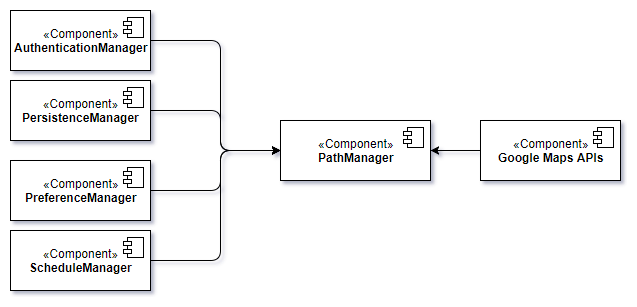
\includegraphics[scale=0.55]{implementation_and_testing/calendar_manager/path.png}
	\end{center}
	\caption{I\&T - PathManager}
\end{figure}

3. \textit{EventManager} is to be integrated with \textit{PersistenceManager}, \textit{AuthenticationManager}, \textit{ScheduleManager} and \textit{PathManager}, following this order no additional drivers or stubs will be needed.
\begin{figure}[H]
	\begin{center}
		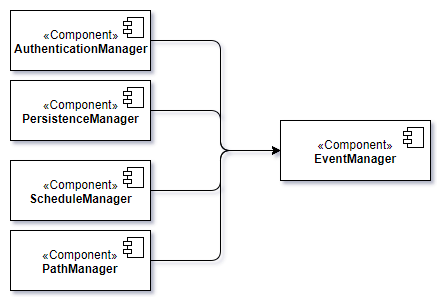
\includegraphics[scale=0.55]{implementation_and_testing/calendar_manager/event.png}
	\end{center}
	\caption{I\&T - EventManager}
\end{figure}

\subsubsection{TripManager}
\textit{TripManager} is to be integrated with \textit{PersistenceManager}, \textit{AuthenticationManager} and then with TSP APIs. Following this order a stub will be needed for the methods of \textit{TSP APIs} called by \textit{TripManager}. The driver needed for this module will simulate user's requests related to the trips-arranging methods provided.
\begin{figure}[H]
	\begin{center}
		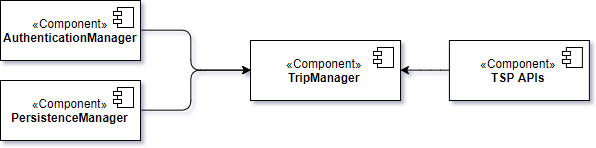
\includegraphics[scale=0.6]{implementation_and_testing/trip.png}
	\end{center}
	\caption{I\&T - TripManager}
\end{figure}

\subsubsection{NotificationManager}
\textit{NotificationManager} interacts only with \textit{GCM APIs} and so it is to be integrated with.
\begin{figure}[H]
	\begin{center}
		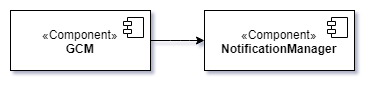
\includegraphics[scale=0.6]{implementation_and_testing/notification.png}
	\end{center}
	\caption{I\&T - NotificationManager}
\end{figure}

\subsubsection{ComplicationManager}
\textit{ComplicationManager} is to be integrated with \textit{PersistenceManager}, \textit{TSP APIs}, \textit{GoogleMaps APIs}, \textit{Weather API's} and \textit{NotificationManager}, following this order a stub will be needed for the methods of \textit{NotificationManager} called by \textit{ComplicationManager} ( basically when \textit{ComplicationManager} will have to notify the user's it will try to forward notification that will be received by the stub).
The integration of the three external APIs can be integrated in any possible order, since the interactions are independent from one another.
\begin{figure}[H]
	\begin{center}
		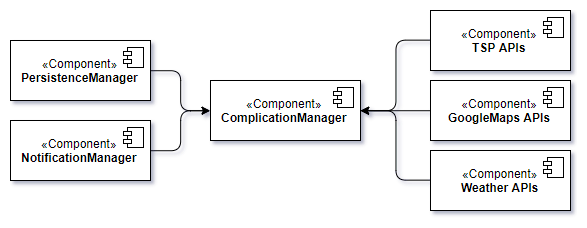
\includegraphics[scale=0.6]{implementation_and_testing/complication.png}
	\end{center}
	\caption{I\&T - ComplicationManager}
\end{figure}

\subsubsection{Overall integration of the Application Server}
The following picture is just a recap of the integration and test plan of the \textit{Application Server}. The integration order starts from the top of the picture and end in the bottom.
\begin{figure}[H]
	\begin{center}
		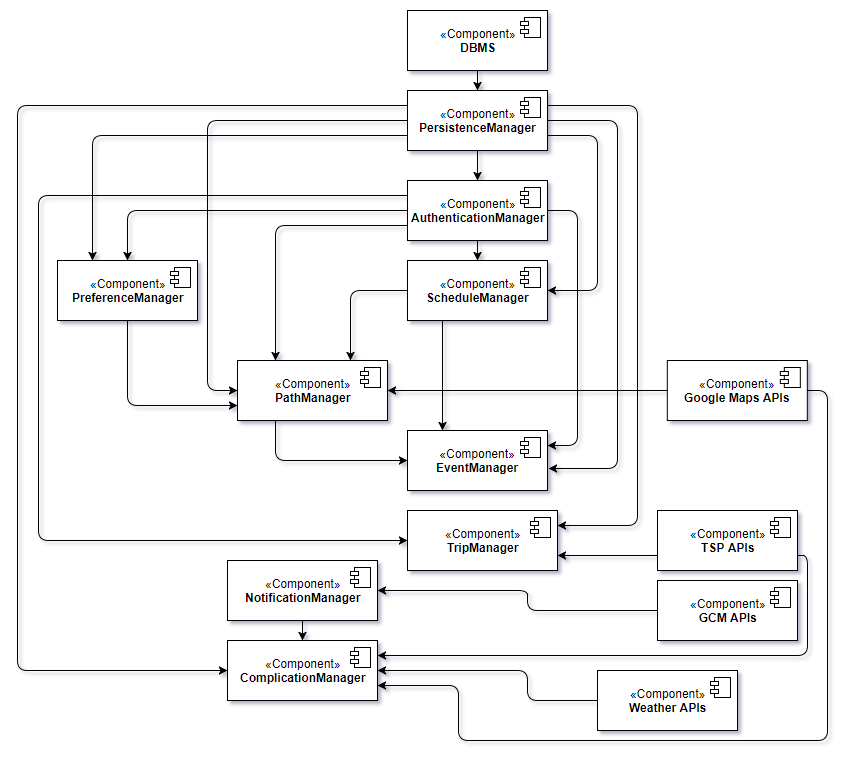
\includegraphics[scale=0.6]{implementation_and_testing/app_server_I&T.png}
	\end{center}
	\caption{I\&T - Application Server}
\end{figure}
\newpage
\subsubsection{WebServer}
In the web server subsystem the \textit{WebController} component is to be integrated with \textit{JavaServerPages} and then with \textit{Google Polylines APIs}. 
\begin{figure}[H]
	\begin{center}
		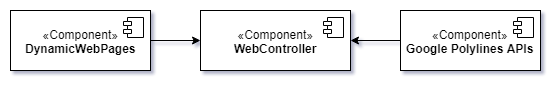
\includegraphics[scale=0.7]{implementation_and_testing/web.png}
	\end{center}
	\caption{I\&T - WebServer}
\end{figure}

\subsubsection{AppMobile}
The order of integration and testing of the \textit{AppMobile}'s components is the following: first \textit{DBManager} with \textit{LocalDBMS} and then \textit{ApplicationController} with \textit{DBManager}, \textit{GUIManager}, \textit{GCM API's} and \textit{Google Polylines APIs}. 
\begin{figure}[H]
	\begin{center}
		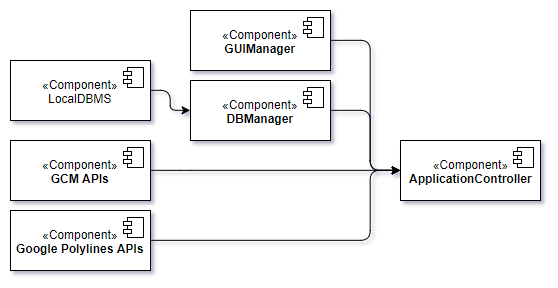
\includegraphics[scale=0.7]{implementation_and_testing/app.png}
	\end{center}
	\caption{I\&T - AppMobile}
\end{figure}
\newpage
\subsection{Subsystems integration Sequence}
Once all subsystem will be fully integrated this is the order in which they are to be integrated together in order to deploy the full Travlendar+ infrastructure.
\begin{figure}[H]
	\begin{center}
		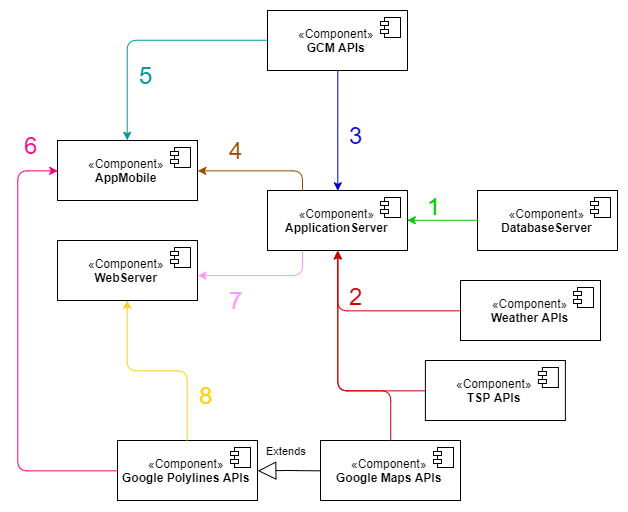
\includegraphics[scale=0.7]{implementation_and_testing/subsystem_integration.png}
	\end{center}
	\caption{I\&T - AppMobile}
\end{figure}
			
	\chapter{EFFORT SPENT}
	\label{ch:EFFORT SPENT}
		\todo{TODO}
	\chapter{REFERENCES}
	\label{ch:REFERENCES}
		\begin{enumerate}[(I)]
	\item \href{https://javaee.github.io/glassfish/doc/5.0/release-notes.pdf}{\color{blue}GlassFish Server Open Source Edition - Release Notes - Release 5.0}
	\item \href{https://javaee.github.io/glassfish/doc/5.0/installation-guide.pdf}{\color{blue}GlassFish Server Open Source Edition - Installation Guide - Release 5.0 }
	\item \href{https://javaee.github.io/glassfish/doc/5.0/installation-guide.pdf}{\color{blue}GlassFish Server Open Source Edition - Installation Guide - Release 5.0 }
	\item Document provided in beep course web page in slides folder: "JEE Tools Instructions for Lab";
\end{enumerate}

\end{document}
